%28/10 - Fátima Sánchez Cabo
\chapter{Introducción a la genómica: caracterización del genoma mediante NGS}
\section{Introducción a la genómica traslacional}
\subsection{Definición e importancia de la genómica}
La genómica, el estudio integral del ADN y de la estructura, función y dinámica de los genomas, representa un pilar fundamental en la biología moderna. Marcó un cambio de paradigma, pasando de un enfoque reduccionista en biología - donde se estudiaban componentes individuales y de manera aislada - a una perspectiva integradora que analiza las interacciones y relaciones entre los distintos elementos biológicos. Esta transición permitió evolucionar de la genética clásica, basada en hipótesis concretas, hacia la genómica, que integra análisis de datos masivos sin necesidad de preguntas iniciales específicas, aunque sí en constante búsqueda de respuestas biológicas complejas.

En el marco del dogma central de la biología, las “ómicas” representan tres niveles de estudio: la genómica (centrada en el ADN), la transcriptómica (ARN) y la proteómica (proteínas). Este curso se enfoca en la genómica, ya que la información genética determina las funciones bioquímicas y, por ende, los fenotipos de los organismos. Gracias a avances recientes, ahora es posible inferir la función bioquímica de las proteínas directamente a partir de la secuencia de ADN, sin necesidad de técnicas complejas como la cristalización. Además, herramientas de inteligencia artificial pueden predecir la estructura de las proteínas con precisión, acelerando la interpretación de funciones biológicas.

Las proteínas, incluyendo enzimas esenciales, son los elementos funcionales clave en la biología. La secuencia de aminoácidos en una cadena polipeptídica define sus propiedades funcionales, y, por tanto, conocer la secuencia genética subyacente (el ADN) facilita predecir la función de una proteína. Aunque determinar experimentalmente las propiedades de una proteína es complejo, la secuenciación genómica ha simplificado enormemente este proceso.

La mejora en tecnologías de secuenciación impulsó el \textbf{Proyecto Genoma Humano}, que logró identificar entre 20,000 y 25,000 genes y determinar la secuencia de los aproximadamente 3 mil millones de pares de bases del genoma humano. Este proyecto también fomentó la creación de bases de datos y herramientas para el análisis de datos genómicos, además de abrir el debate sobre los aspectos éticos, legales y sociales (conocidos como ELSI, por sus siglas en inglés), que siguen siendo temas vigentes y complejos en la actualidad.

\paragraph{Evolución de la bioinformática en la genómica}
La bioinformática ha crecido a la par de la genómica en múltiples niveles. Inicialmente, era una \textbf{disciplina} incipiente y se desarrollaba como apoyo experimental; sin embargo, ha evolucionado hasta convertirse en un campo esencial que impulsa la investigación. En cuanto a su \textbf{material, los datos,} la bioinformática ha tenido que adaptarse al fenómeno del big data, pasando de manejar cantidades limitadas de datos a enfrentar volúmenes masivos, propios de la genómica actual. Paralelamente, el \textbf{rol de los bioinformáticos} se transformó, pasando de ser técnicos a científicos de datos y académicos altamente reconocidos en la industria y en la investigación.

\begin{figure}[htbp]
\centering
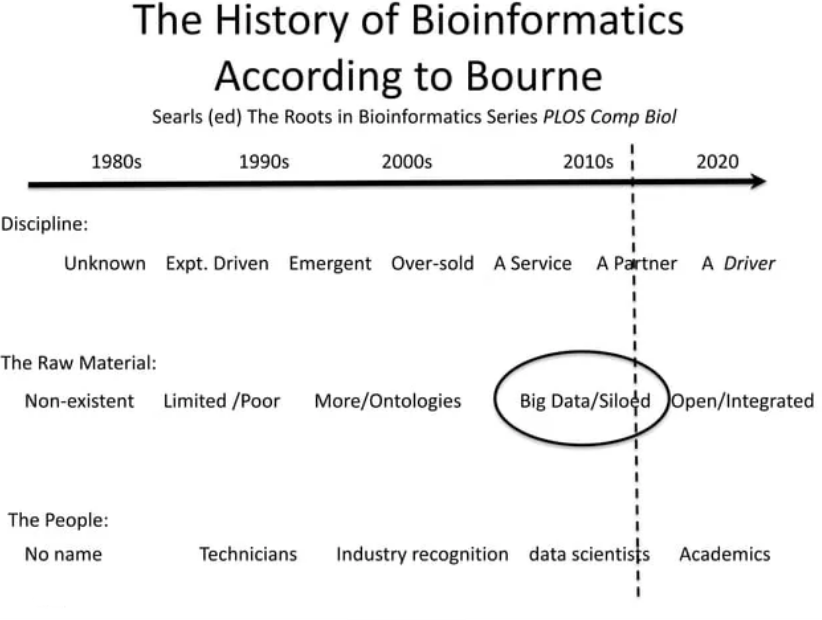
\includegraphics[width = 0.5\textwidth]{figs/history-bioinfo.png}
\caption{Breve historia de la bioinformática en tres niveles: como disciolina, como material que utiliza y como las personas que trabajan en ella. Evolución desde 1980 hasta 2020.}
\end{figure}

\subsection{Avances tecnológicos en secuenciación}
Existen distintos tipos de tecnologías de secuenciación, comúnmente clasificadas en tres generaciones: la primera generación (first generation), la segunda o Next Generation Sequencing (NGS) y la tercera generación. Las dos primeras generaciones se enfocan en la secuenciación de fragmentos cortos de ADN, mientras que la tercera generación permite la lectura de fragmentos largos, facilitando el ensamblaje completo de genomas. Actualmente, uno de los mayores desafíos tecnológicos es detectar variantes de baja frecuencia y realizar secuenciaciones de ADN en células individuales (single-cell sequencing), lo cual tradicionalmente se hacía de forma masiva (“bulk”).

\begin{figure}[htbp]
\centering
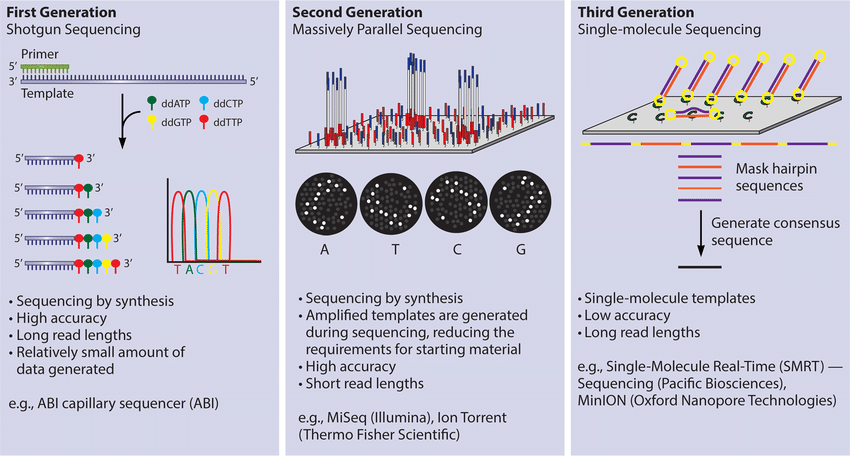
\includegraphics[width = 0.7\textwidth]{figs/sequencing-generations.png}
\caption{Las tres generaciones de secuenciación y su forma de actuar.}
\end{figure}

A medida que el costo de la secuenciación ha disminuido y la capacidad de almacenamiento ha mejorado desde 1990, los datos generados también han crecido exponencialmente. En un experimento de secuenciación, los costos abarcan tanto la secuenciación en sí como el procesamiento bioinformático, el reporte y el almacenamiento de los datos. La comunidad científica y muchos journals requieren que los datos de proyectos financiados públicamente estén disponibles en bases de datos accesibles, lo que asegura la transparencia y el acceso a esta información valiosa. Para obtener una cobertura de calidad, el ADN suele secuenciarse al menos 30 veces, lo que genera archivos de gran tamaño, como los archivos FastQ, que almacenan información de secuencia y calidad para cada base.

\subsection{Procesos de llamada y priorización de variantes}
Los datos de secuenciación se procesan en pipelines bioinformáticas que comienzan con archivos FastQ normalmente comprimidos y pasan por varias etapas: control de calidad, alineamiento y llamada de variantes (variant calling). Las variantes identificadas pueden incluir cambios de nucleótidos, variaciones en el número de copias de segmentos genómicos (copy number variation) o reordenamientos estructurales.

\begin{figure}[htbp]
\centering
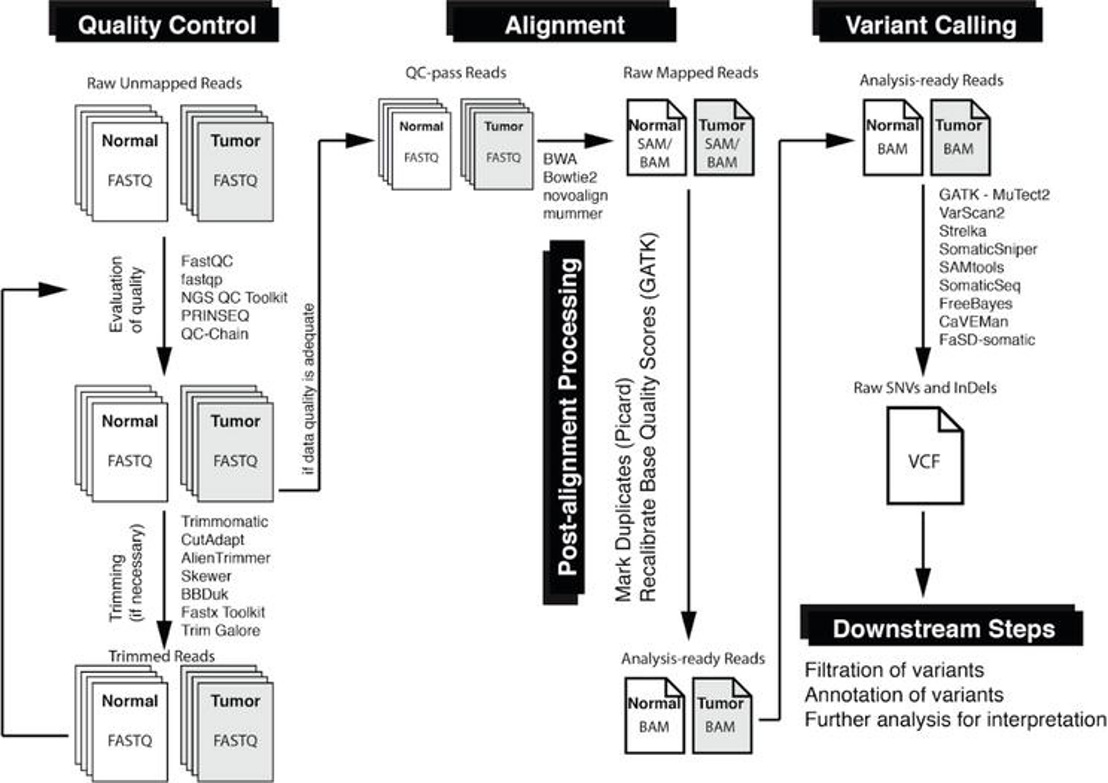
\includegraphics[width = 0.7\textwidth]{figs/bioinfo-pipeline.png}
\caption{Esquema de la pipeline que se sigue en bioinformática para la llamada de variantes.}
\end{figure}

La priorización de variantes se basa en factores como el impacto funcional, la frecuencia alélica en la población y la asociación con enfermedades. Sin embargo, muchas variantes requieren validación experimental, frecuentemente en modelos animales como ratones, para corroborar su relevancia funcional. El proceso de filtrado inicial se enfoca en variantes en exones de genes candidatos, analizando su frecuencia, patogenicidad y modelo de herencia; en caso de no hallarse variantes relevantes, se amplía el análisis a variantes oligogénicas o no codificantes.

\begin{figure}[htbp]
\centering
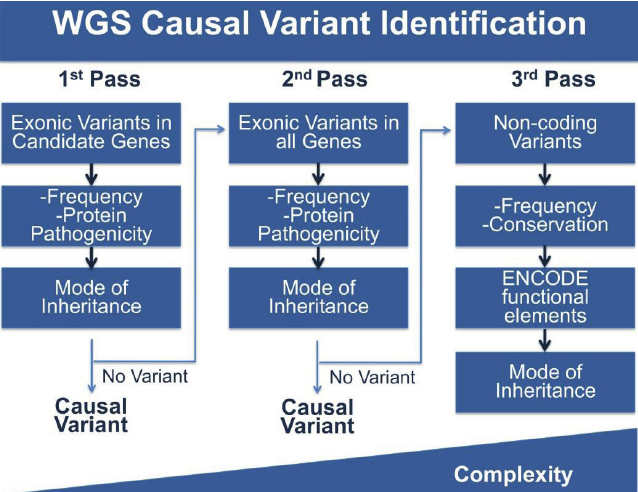
\includegraphics[width = 0.5\textwidth]{figs/variant-priorization.png}
\caption{Ejemplo de la priorización de variantes.}
\end{figure}

\subsection{Genómica en medicina de precisión}
La genómica ha transformado el enfoque de la medicina de precisión, permitiendo identificar enfermedades con bases genéticas, ambientales o una combinación de ambas. Algunas variantes genéticas confieren una predisposición a enfermedades sin ser causantes directas, lo cual es crucial para inferir relaciones causales y acelerar ensayos clínicos mediante la integración de grandes volúmenes de datos. Estas variantes pueden clasificarse en germinales (heredadas) o somáticas (adquiridas).

\begin{figure}[htbp]
\centering
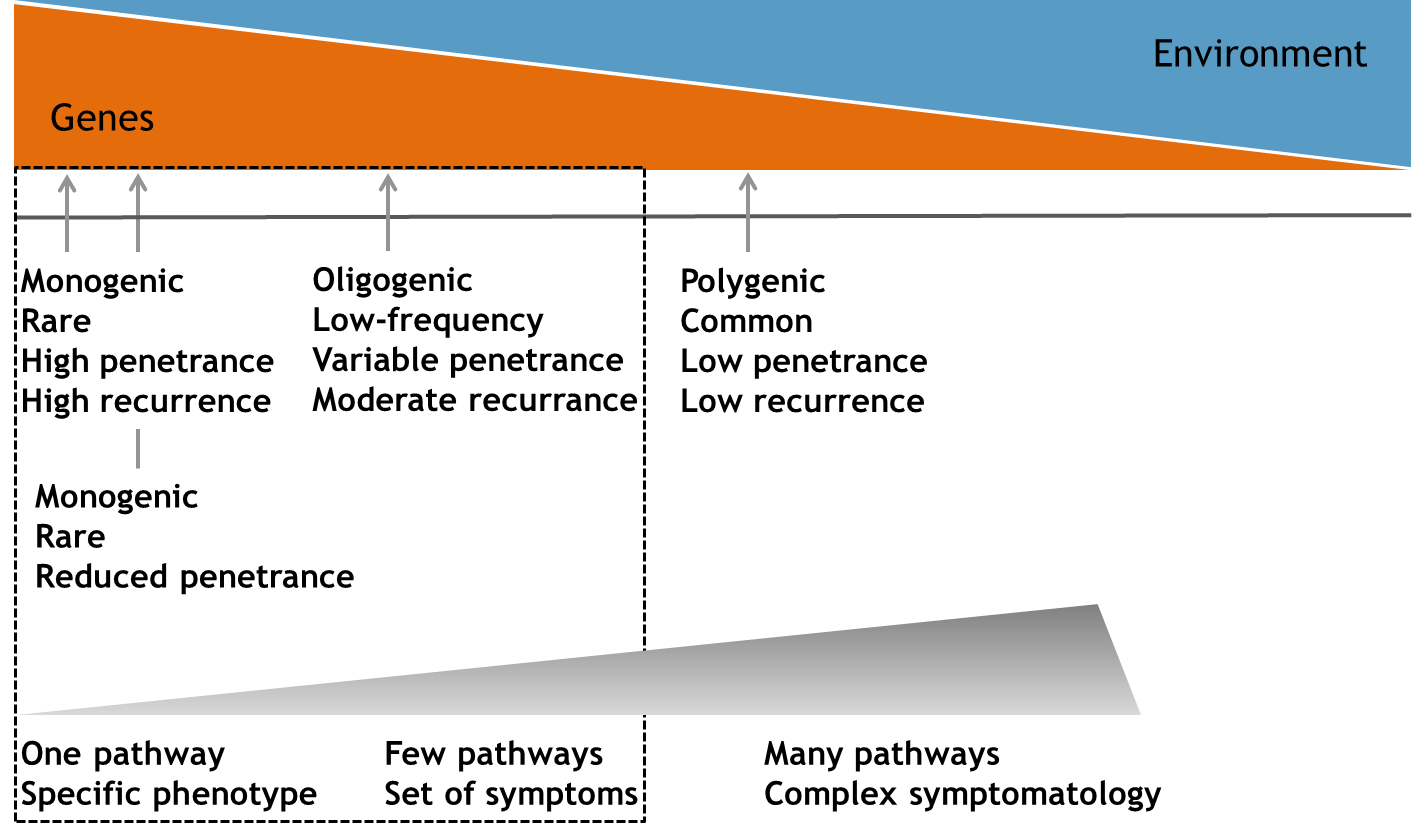
\includegraphics[width = 0.5\textwidth]{figs/genetic-environment.png}
\caption{Representación gráfica de la relación entre enfermedades con base genética, ambientales o una mezcla de ambas.}
\end{figure}

En medicina de precisión, la genómica es solo una capa de datos entre muchas. Para una comprensión holística de la salud y la enfermedad, es necesario combinarla con información de otras “ómicas” como la transcriptómica, epigenómica, proteómica, metabolómica, y datos de microbioma. Además, los datos clínicos y epidemiológicos también forman parte del ecosistema de \textbf{Big Data Biomédico}, que actualmente se maneja mediante técnicas avanzadas de computación en clusters HPC, computación en la nube y algoritmos de GPU.

\begin{figure}[htbp]
\centering
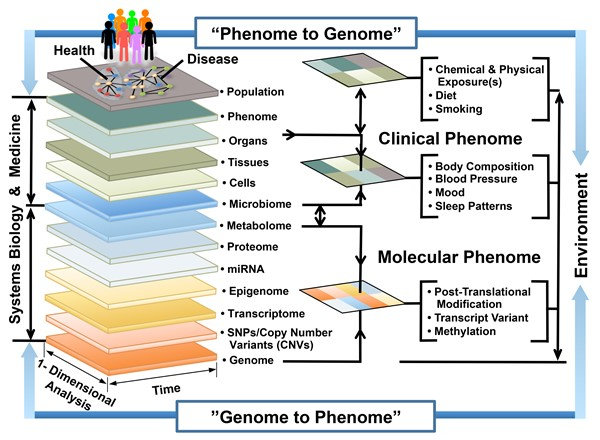
\includegraphics[width = 0.7\textwidth]{figs/bigger-picture-bioinfo.jpg}
\caption{Esquema representando el dibujo general de la bioinformática.}
\end{figure}

Varias bases de datos públicas permiten estudiar la transición entre salud y enfermedad. El estudio de Farmingham, por ejemplo, lleva más de 70 años recolectando datos de factores de riesgo cardiovascular en más de 15,000 participantes. En Reino Unido, el Biobank y, en Estados Unidos, la iniciativa All of Us, también representan recursos de gran envergadura. En España, el CNIC (Centro Nacional de Investigaciones Cardiovasculares) realiza el estudio PESA (Progression of Early Subclinical Atherosclerosis), que ha contribuido a identificar factores predictivos de aterosclerosis subclínica mediante el estudio multiómico, generando nuevos indicadores con un mayor poder predictivo de la formación de placas de colesterol.

\paragraph{Epigenética y la medición de la edad biológica}
El perfil de metilación del ADN es un factor epigenético que puede modificar la expresión genética y se ha utilizado para calcular la “edad biológica” o epigenética de una persona, lo que puede servir como predictor de esperanza de vida y salud. Al comparar estos perfiles con la edad cronológica, sexo y otros factores, se obtiene información sobre el envejecimiento y el riesgo de enfermedades, facilitando el desarrollo de estrategias de salud personalizadas.

\subsection{Resumen}
La genómica ha liderado una revolución científica en el siglo XX, evolucionando desde el estudio de componentes individuales hasta una perspectiva integral de sistemas biológicos y de investigación basada en datos masivos. La bioinformática se ha convertido en una disciplina central en el análisis genómico y predicción de estructuras proteicas, impulsada por el Proyecto Genoma Humano y el desarrollo de tecnologías de secuenciación. Los avances actuales buscan no solo la secuenciación del ADN, sino también la integración de estos datos con datos epidemiológicos y moleculares para obtener una comprensión más profunda de la salud y la enfermedad. Así, el Proyecto Genoma Humano fue decisivo para sentar las bases de tecnologías de secuenciación, el desarrollo de la bioinformática en sí y el uso social e industrial de los datos ómicos.

La identificación de características genómicas relevantes causales de rasgos/enfermedades se basa en la anotación de variantes en bases de datos y en estudios poblacionales: hay margen de mejora y un gran éxito de la ciencia colaborativa. Hoy en día, los principales proyectos tratan no sólo de secuenciar el ADN, sino de integrar esta información con datos epidemiológicos y otros datos moleculares para comprender mejor la salud y la enfermedad.
Las enfermedades, en función de su base genética, pueden clasificarse en monogénicas (mendelianas), oligogénicas (ej., cardiopatías familiares) y complejas (evaluadas mediante puntuaciones de riesgo poligénicas). Esta clasificación permite avanzar en la medicina de precisión, abordando enfermedades desde su origen genético para ofrecer intervenciones de salud más efectivas y personalizadas.

%30/10 - Álvaro Serrano
\section{Métodos de secuenciación}
La secuenciación permite pasar de la información contenida en el ADN a un dominio digital mediante una representación abstracta. 

El primer método de secuenciación fue el \textbf{método Maxam-Gilbert}, que utilizaba un marcador en el extremo 5' del ADN. En este proceso, el ADN se trataba con diferentes compuestos químicos para provocar rupturas específicas en función de cada base nitrogenada. Los fragmentos resultantes se separaban en un gel de acrilamida mediante electroforesis, y se revelaban mediante autoradiografía de rayos X. La secuencia se deducía observando el patrón de bandas resultante.

\begin{figure}[htbp]
\centering
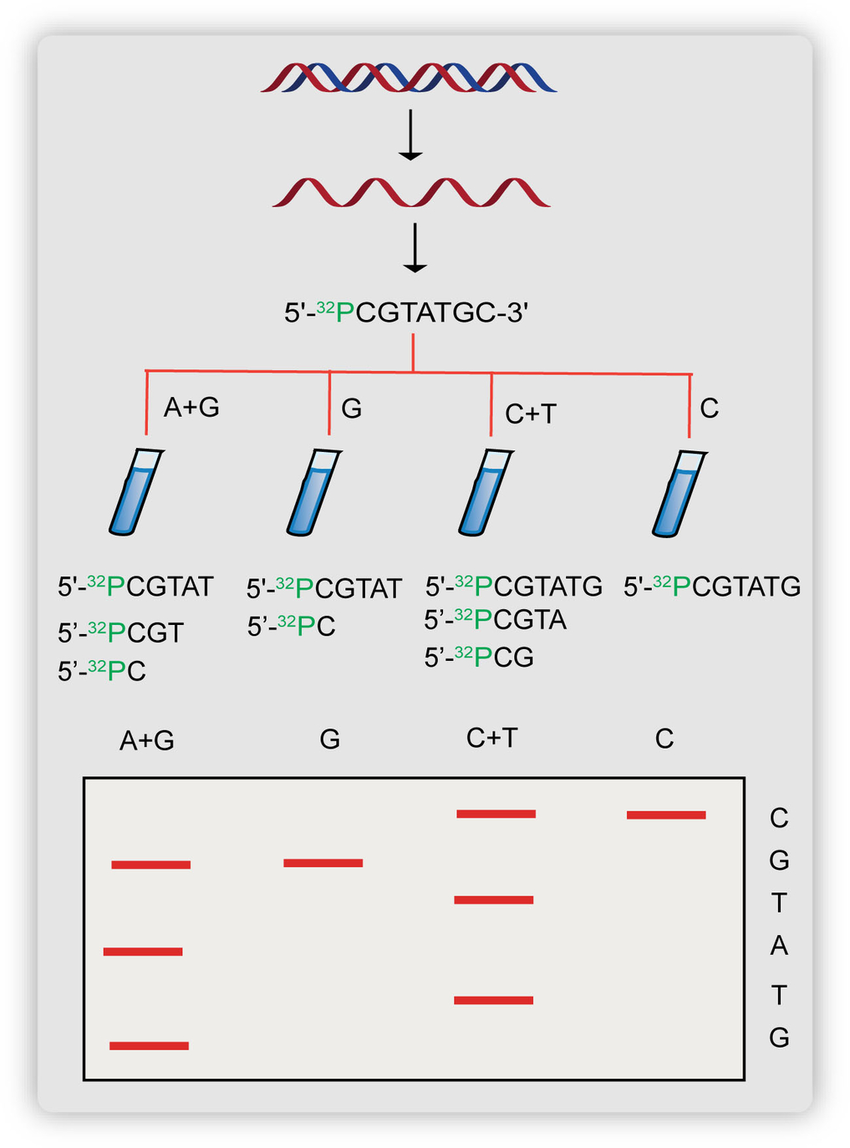
\includegraphics[width = 0.3\textwidth]{figs/maxam-gilbert.png}
\caption{\textbf{Principio de la secuenciación Maxam-Gilbert}: Se llevaron a cabo cuatro reacciones separadas para la degradación de bases en un fragmento de ADN monocatenario: A+G, G, C+T y C. Se obtienen fragmentos de ADN de diferente longitud tras la degradación de las bases y la escisión del esqueleto de azúcar-fosfato. Los productos se cargan en cuatro pocillos separados de un gel de poliacrilamida. La secuencia se lee de abajo a arriba como GTATGC. Si se encuentra una G frente a un hueco en el gel, se confirma que se trata de 5-metilcitosina en la cadena molde.}
\end{figure}

Otro método clave es el de \textbf{terminación de cadena, o método de Sanger}. Este utiliza deoxinucleótidos modificados, que tienen un átomo de hidrógeno en el grupo 2' de la pentosa, en lugar de un grupo hidroxilo (OH). Esto impide la unión del extremo 5' al 3', deteniendo así la extensión de la cadena de ADN. El resultado es una mezcla de fragmentos de distintos tamaños, los cuales se marcan con isótopos radioactivos o, en versiones más modernas, con fluoróforos. La secuencia se obtiene mediante detección de colores en una única reacción, simplificando el análisis. La clave de este método \marginpar[\footnotesize Pregunta examen] \ es el uso de dideoxinucleótidos, que interrumpen la actividad de la ADN polimerasa, permitiendo detener la cadena de manera controlada.

\begin{figure}[htbp]
\centering
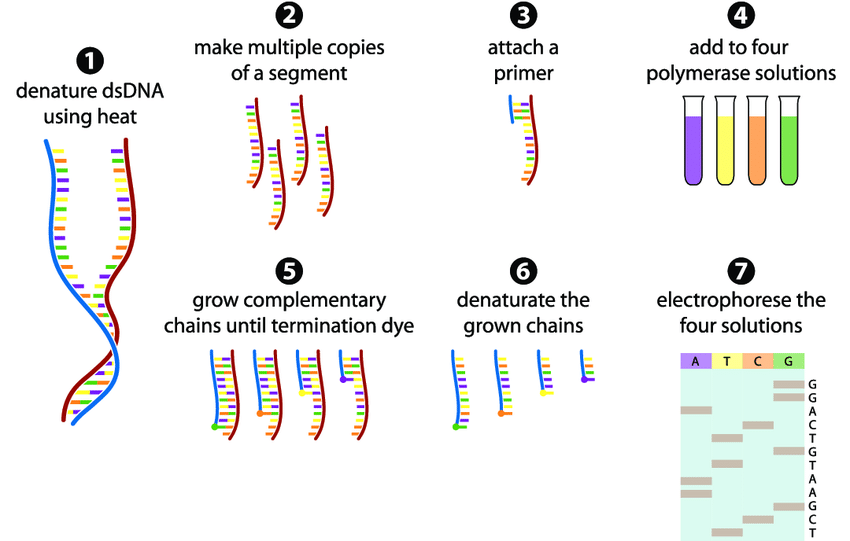
\includegraphics[width = 0.8\textwidth]{figs/sanger.png}
\caption{\textbf{El método de secuenciación Sanger en 7 pasos.} (1) El fragmento de dsADN se desnaturaliza en dos fragmentos de ssADN. (2) Un fragmento de ssADN se multiplica en millones de copias. (3) Se une un cebador que corresponde a un extremo del fragmento. (4) Los fragmentos se añaden a cuatro soluciones de polimerasa. Cada solución contiene los cuatro tipos de bases pero sólo un tipo de nucleótido de terminación. (5) La cadena crece hasta que se añade aleatoriamente un nucleótido de terminación. (6) Los fragmentos de dsADN resultantes se desnaturalizan para obtener una serie de ssADN de distintas longitudes. (7) Los fragmentos se separan por electroforesis y se lee la secuencia.}
\end{figure}

El primer secuenciador automático fue el ABI370, capaz de secuenciar hasta 5000 bases al día. Sin embargo, se necesitarían aproximadamente 16,000 años para secuenciar todo el genoma humano usando esta tecnología. Este secuenciador innovador reemplazaba los geles por electroforesis capilar y un detector de fluorescencia. Durante el Proyecto Genoma Humano en los años 90 y 2000, desarrollado en colaboración entre el sector público y privado, se introdujeron mejoras significativas a los secuenciadores, como el modelo ABI377, que empleaba varios capilares para incrementar la eficiencia. Sin embargo, la secuenciación de regiones altamente repetitivas del genoma, como los telómeros y centrómeros, fue compleja, y la primera descripción completa del genoma humano fue publicada hace apenas un año.

\subsection{Métodos de secuenciación empleados en el Proyecto Genoma Humano}
Los métodos que se utilizaron en el proyecto fueron los siguientes:
\begin{itemize}
\item \textbf{Hierarchical Shotgun:} En este método, el ADN se clona en fragmentos más pequeños usando enzimas de restricción. Estos fragmentos se solapan y forman contigs, los cuales se ensamblan progresivamente para reconstruir la secuencia original.
\item \textbf{Whole-genome Shotgun:} Similar al método anterior, pero se realiza directamente sobre el genoma completo en lugar de partir de cromosomas bacterianos. El ADN se clona en bacterias, se fragmenta y se ensamblan los contigs mediante solapamiento.
\end{itemize}

\begin{figure}[htbp]
\centering
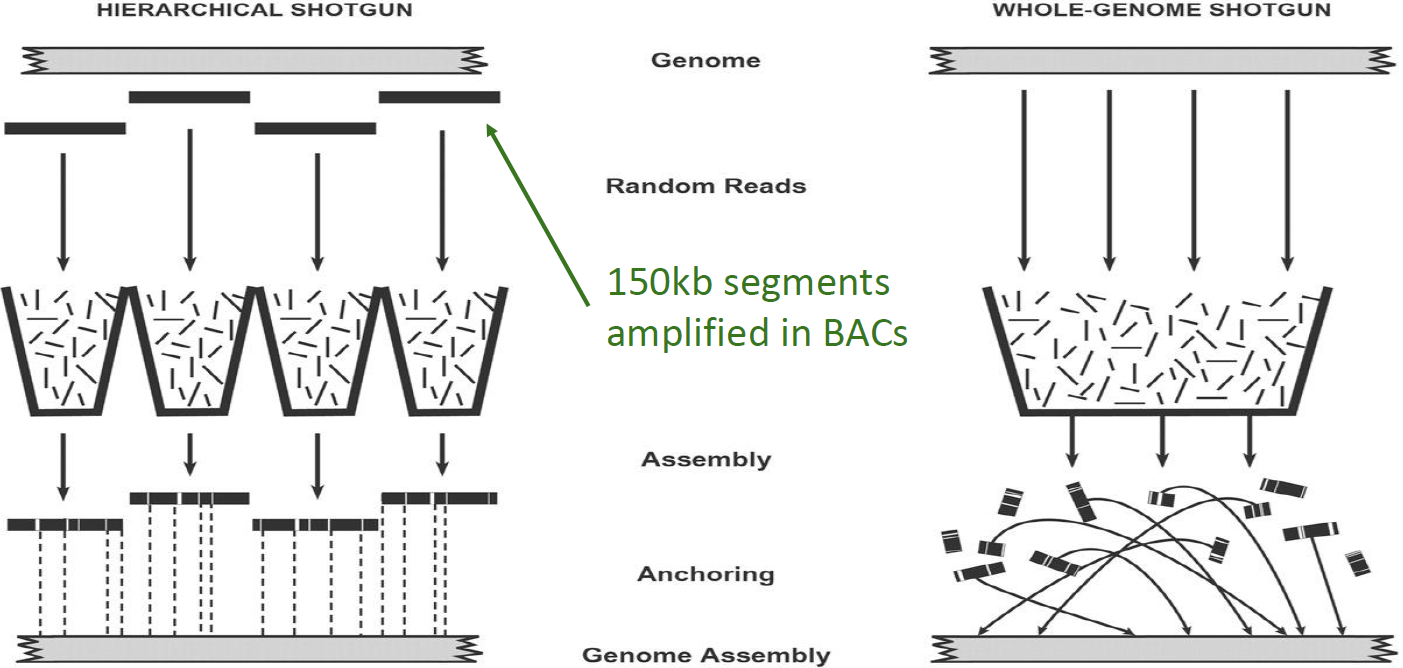
\includegraphics[width = 0.8\textwidth]{figs/HGP-sequencing.png}
\caption{\textbf{Estrategias de secuenciación en el Proyecto Genoma Humano.} (Izquierda) La estrategia de hierarchical shotgun (HS) consiste en descomponer el genoma en un camino de mosaico de clones BAC (bacterial artificial chromosome) superpuestos, realizar la secuenciación en cada BAC y volver a ensamblarlo, y luego fusionar las secuencias de clones adyacentes. El método tiene la ventaja de que todos los contigs de secuencias y scaffolds derivados de un BAC pertenecen a un único compartimento con respecto al anclaje al genoma. (Derecha) La estrategia WGS (Whole-genome shotgun) consiste en secuenciar todo el genoma e intentar reensamblar toda la colección. Con el método WGS, cada contig y scaffold es un componente independiente que debe anclarse al genoma. En general, muchos scaffolds no pueden anclarse sin esfuerzos dirigidos. (Los contigs son bloques contiguos de secuencia; los scaffolds son conjuntos de contigs unidos por lecturas emparejadas de ambos extremos de un inserto plasmídico).}
\end{figure}

La electroforesis capilar, usada en ambos métodos, permite separar fragmentos de ADN de diferentes tamaños a través de un capilar con un detector de fluorescencia, logrando una lectura precisa de aproximadamente 500 pares de bases por fragmento. Con el tiempo, los costos de secuenciación disminuyeron gracias a avances en técnicas posteriores al método de Sanger.

\subsection{NGS: la siguiente generación de tecnología de secuenciación del ADN}
La secuenciación de segunda generación o Next-Generation Sequencing (NGS) permite una secuenciación paralela y masiva, también conocida como \textbf{high-throughput sequencing}. Los principales métodos NGS incluyen 454 Roche, Solexa Illumina, ABI/SOLiD, Complete Genomics, Pacific Biosciences, Ion Torrent y Oxford Nanopore.

\subsubsection{Preparación de librerías de NGS}
Las librerías de secuenciación se preparan fragmentando el ADN y generando secuencias que luego se amplifican y procesan en el secuenciador, obteniendo las lecturas o reads. Estas librerías se amplifican clonalmente mediante tres métodos:
\begin{itemize}
\item \textbf{Beads:} pequeñas bolitas recubiertas de primers, donde el ADN se adhiere y se amplifica.
\item \textbf{Fase sólida:} el ADN se adhiere a una superficie de cristal donde se amplifica.
\item \textbf{Nanobolas:} se produce un ovillo de ADN amplificado en forma circular, que se adhiere a una placa metálica funcionalizada (con grupos funcionales) para secuenciación.
\end{itemize}

La secuenciación NGS utiliza un gran número de moléculas idénticas, permitiendo una secuenciación paralela de alta eficiencia y alto rendimiento o high-throughput. La característica de la segunda generación es que utiliza la molécula de ADN original y, sobre ella, la amplifica, es decir, la utiliza como molde para generar muchas moléculas iguales. 

\subsubsection{Clasificación de NGS: secuenciación por síntesis y por ligación}
Los métodos de secuenciación de segunda generación se pueden clasificar en secuenciación por síntesis (con la enzima polimerasa) o secuenciación por ligación (con la enzima ligasa).

\begin{itemize}
\item \textbf{Secuenciación por síntesis (SBS)}
\begin{itemize}
\item \textbf{Ciclo de terminación reversible (CRT):} una evolución del método Sanger. Se utiliza ADN unido a beads o cristales y se añaden dNTPs modificados con el grupo 3’ OH bloqueado, limitando así la duplicación de la polimerasa. Cada ciclo implica la incorporación de un nucleótido, seguido de una señal fluorescente específica del nucleótido unido. Posteriormente, el grupo OH se desbloquea con un químico de lavado para que el proceso continúe. La señal que se detecta no es de un único nucleótido, si no del conjunto de nucleótidos del cluster, que debido a la amplificación clonal, debería ser la misma señal amplificada. Esto se realiza por el límite de detección de fluorescencia de los microscopios. Además, la placa con los moldes tiene en los límites unos marcadores que permiten que el microscopio se enfoque a la altura a la que debe. 

\begin{figure}[htbp]
\centering
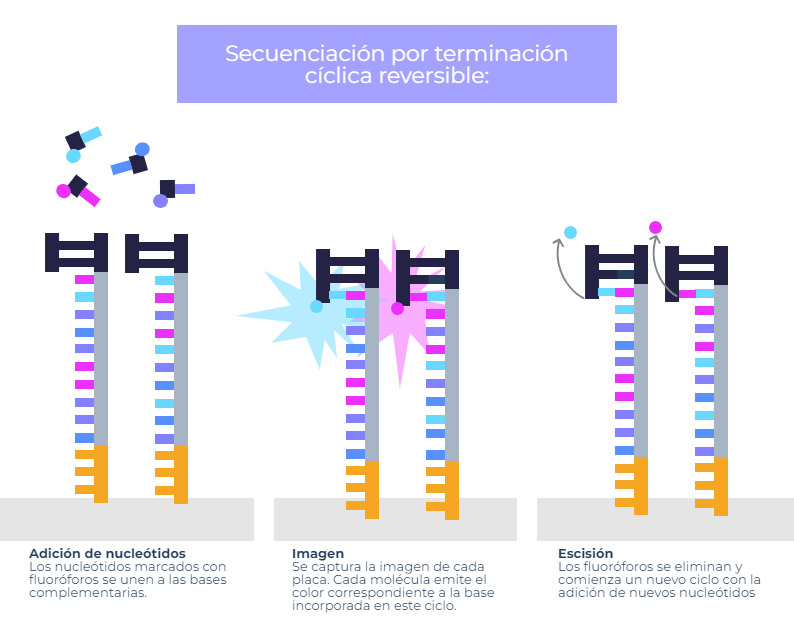
\includegraphics[width = 0.7\textwidth]{figs/secuenciacion-terminacion-ciclica-reversible.jpg}
\caption{\textbf{Secuenciación por terminación cíclica reversible:}
Esta metodología se basa en la utilización de nucleótidos marcados con fluoróforos en una reacción de síntesis de ADN. Cada vez que uno de estos nucleótidos se incorpora a la cadena, el sistema toma una captura y registra de qué tipo de nucleótido se trata. Una vez tomada la captura, se eliminan los fluoróforos de los nucleótidos que se han incorporado y se continúa la síntesis de la cadena con nuevos nucleótidos marcados. }
\end{figure}

Una vez terminada la secuenciación, se utiliza como primer para secuenciar la cadena contraria. Esto se debe a que el microscopio va enfocando peor y se pierde calidad. Cada señal emitida por el fluoróforo se conoce como call o llamada. Cada call tiene una confident score de Q, que se calcula mediante la fórmula $Q = - 10 \cdot log_{10} P $. Por tanto, si Q es 30, P sería $10^{-3}$, representando P la probabilidad de error. La información que se obtiene en el archivo es la secuencia obtenida con un valor Q asociado codificado en ASCII. 

Los microscopios se clasifican en microscopios de 4 canales y de 2 canales. Los microscopios de 4 canales tienen una mayor calidad al poder distinguir cada uno de los nucleótidos, mientras que los de 2 canales utilizan la combinación de dos fluoróforos: se detecta verde, rojo, la combinación entre verde y rojo, y la ausencia de fluorescencia. Esto último es algo arriesgado, ya que algunos nucleótidos podrían perder el fluoróforo y se consideraría ausencia de fluorescencia. No obstante, estos microscopios de 2 canales, pese a tener una peor calidad, son más rápidos y baratos. Respecto al secuenciador, hay varios tipos, por lo que al elegir uno se tendrá que tener cuenta el caso de uso y el dinero disponible (la página de Illumina tiene tablas comparativas para elegir el mejor secuenciador para cada caso). 

\begin{figure}[htbp]
\centering
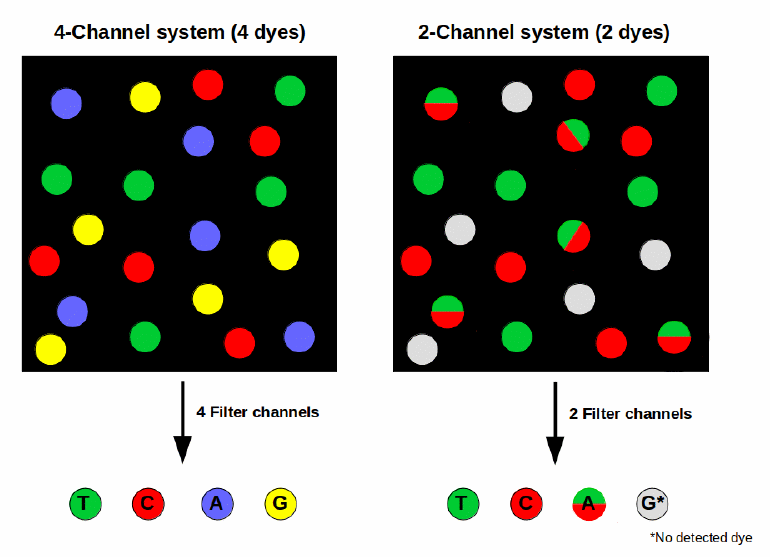
\includegraphics[width = 0.7\textwidth]{figs/microscope-channels.png}
\caption{Comparación entre los microscopios de 4 y de 2 canales.}
\end{figure}

Las ventajas de la secuenciación CRT es que es la que produce la mayor cantidad de secuencias secuenciadas a la vez (mayor throughput). La desventaja es el límite que puede secuenciar, que es en torno a 150 bases por cada extremo. 

\item \textbf{Adición de nucleótidos simple (SNA):} en cada ciclo se añade un solo tipo de nucleótido, detectando su incorporación. Este método es sensible a los homopolímeros (repeticiones del mismo nucleótido), lo que puede generar problemas de fase si la señal no es proporcional al número de nucleótidos añadidos.
\begin{itemize}
\item \textbf{Pirosecuenciación:} emplea pirofosfato liberado en la síntesis de ADN. Debido a su enlace de alta energía, la acción de la pirofosfatasa acoplada a la luciferasa produce que se emita una señal de luz proporcional al número de nucleótidos añadidos. Este método es rápido, económico y preciso, aunque presenta limitaciones con secuencias largas debido al cambio de fase en el momento en el que se produzca un error. La calidad de la secuenciación es Q45 (99,997\%). 

\begin{figure}[htbp]
\centering
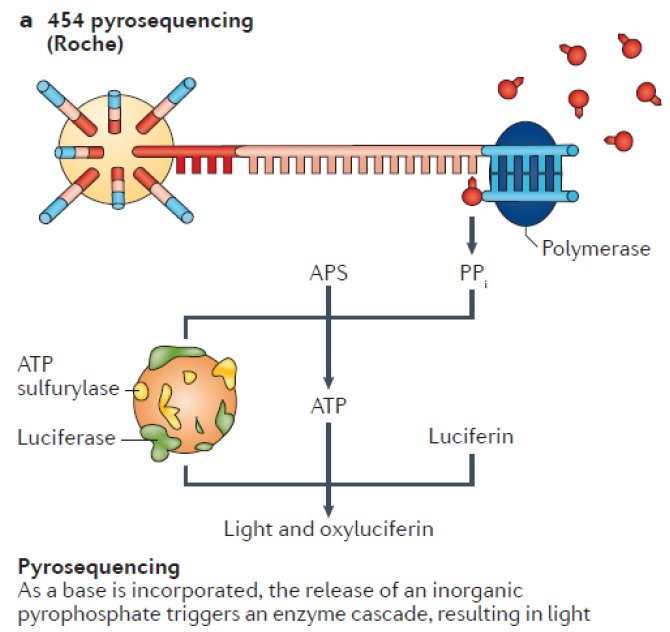
\includegraphics[width = 0.5\textwidth]{figs/pirosecuenciacion.png}
\caption{Esquema de la pirosecuenciación, tecnología que permite determinar el orden de una secuencia de ADN mediante luminiscencia.}
\end{figure}

\item \textbf{Ion Torrent proton detection:} mide el cambio de pH (cambio de potencial) que ocurre al liberar un protón durante la polimerización del ADN. Al final de cada ciclo es necesario lavar para evitar la señal cruzada. La técnica es económica y ampliamente utilizada en hospitales, pero presenta desafíos con secuencias largas debido a la falta de proporcionalidad en la señal en secuencias con regiones muy repetitivas (si se unen dos nucleótidos en lugar de uno, la señal es proporcional a los dos, pero cuando se unen 50 nucleótidos, el cambio de potencial no es proporcional a los 50).

\begin{figure}[htbp]
\centering
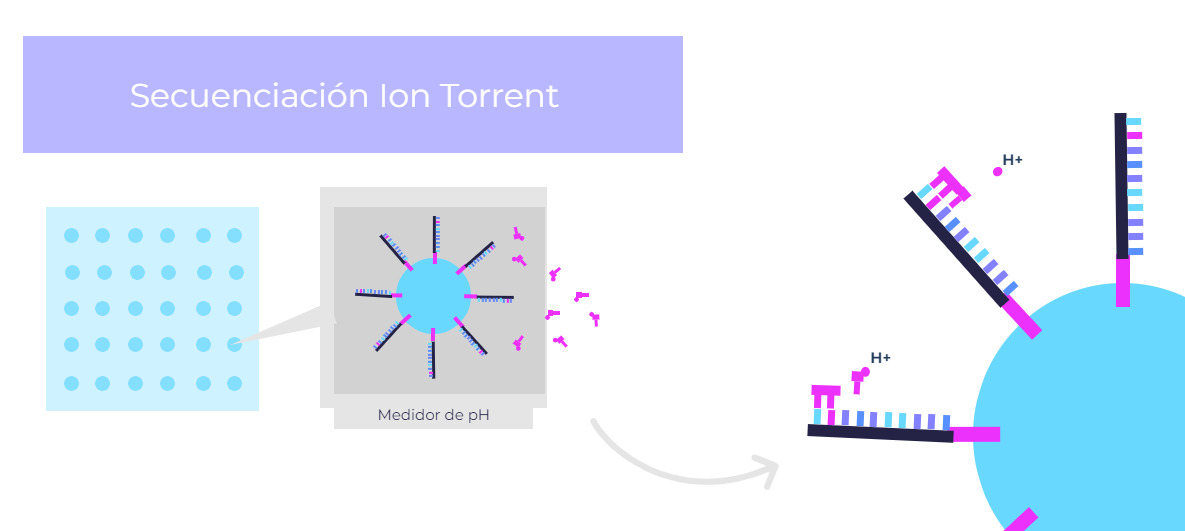
\includegraphics[width = 0.7\textwidth]{figs/Ion-torrent-sequencing.jpg}
\caption{\textbf{Secuenciación por Ion Conductor (Ion Torrent Sequencing):} 
Se trata de una estrategia que se basa en la detección de las modificaciones en el pH que se producen en la síntesis de ADN. Para ello, se van incorporando nucleótidos a una cadena de ADN, provocando que se libere un protón (H+) en la reacción y, por tanto, que se vea modificado el pH. Para poder diferenciar cuál de los cuatro tipos de nucleótidos se ha introducido en cada posición de la secuencia, se repiten varios ciclos, cada uno de ellos, con la adición de un único tipo de nucleótido. }
\end{figure}

\end{itemize}
\end{itemize}

\item \textbf{Secuenciación por ligación (SBL)}
\begin{itemize}
\item \textbf{Secuenciación por SOLiD:} Este método emplea sondas de ligación con dos bases complementarias a la base que se secuencia. En cada ciclo, una ligasa une una sonda marcada con un fluoróforo y luego se elimina la fluorescencia para repetir el ciclo, generando datos precisos, aunque menos comunes en la práctica. Se van mapeando dos nucleótidos a la vez, dejando un espacio de 3 nucleótidos. Por ello, se repite cinco veces añadiendo espaciadores que permitan el solapamiento de las lecturas.

\begin{figure}[htbp]
\centering
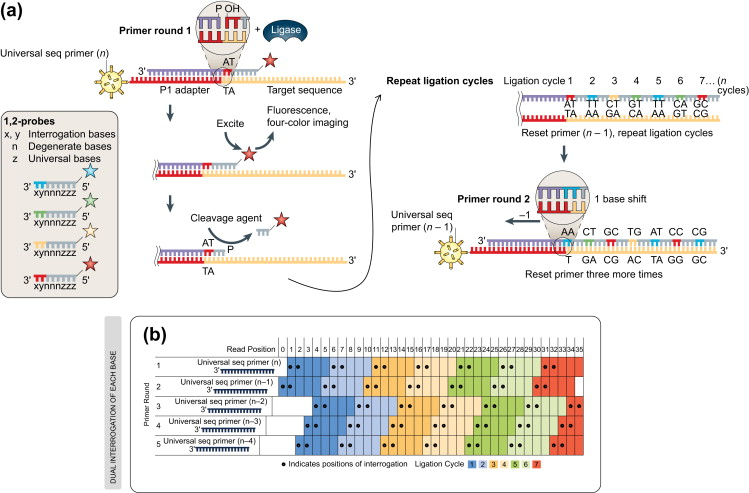
\includegraphics[width = \textwidth]{figs/solid-sequencing.jpg}
\caption{\textbf{Ilustración del método de secuenciación por ligación utilizando la plataforma SOLiD.} (a) Esquema de los diferentes pasos seguidos por el método SOLiD de ligadura por cuatricromía: hibridación de primers, ligadura selectiva de las sondas, obtención de imágenes por cuatricromía y escisión de la sonda. El ciclo SOLiD se repite nueve veces más. El producto de extensión se elimina y la plantilla se reajusta con un cebador complementario a la posición n -1 para una segunda ronda de ciclos de ligación. (b) Se realizan cinco rondas de reajuste del cebador para cada etiqueta de secuencia. Mediante el procedimiento de reajuste de cebadores, prácticamente todas las bases se consultan en dos reacciones de ligación independientes con dos cebadores diferentes.}
\end{figure}

\item \textbf{Complete Genomics (Nanoballs, BGI):} Amplifica ADN mediante rolling circle para formar ovillos, que luego se hibridan en una placa. Las sondas fluorescentes hibridan de forma iterativa para secuenciar el ADN. Este método permite una alta densidad de secuencias pequeñas, teniendo así una precisión muy alta. No obstante, permite secuenciar lecturas pequeñas y, al final, se utilizan distintos adaptadores a los que se unen las sondas, permitiendo aumentar el througput. Hay partes de la tecnología que no se conocen y está principalmente disponible en China.
\end{itemize}
\end{itemize}

\subsubsection{Limitaciones y desafíos en NGS}
La NGS de segunda generación presenta una tasa de error de Q25-Q35 y ciertas limitaciones:
\begin{itemize}
\item \textbf{Lecturas cortas} generan dificultades en el ensamblaje de genomas completos y en la identificación de variantes estructurales.
\item \textbf{Errores de secuenciación} especialmente en regiones complejas y repetitivas, como secuencias AT/GC (SBS) y homopolímeros (SNA).
\item \textbf{Sesgo de amplificación} algunas regiones se amplifican mejor que otras, afectando la uniformidad en las lecturas.
\item \textbf{Alto coste de los equipos}
\item \textbf{Fenómeno de la cadena retrasada} cuando no se incorpora un nucleótido, produciendo un descabalgamiento del ciclo de lectura real y el ciclo de lectura en el que creemos que estamos.
\item \textbf{Persistencia de errores en los cluster} al producirse un error en el cluster, el error se queda a lo largo de la secuenciación.
\item \textbf{Cambios epigenéticos}
\end{itemize}

\subsection{Resumen}
La secuenciación ha cambiado la forma de hacer y entender la biología. La secuenciación de segunda generación o NGS permite secuenciar millones de moldes de ADN al mismo tiempo. Generalmente, el molde de ADN es amplificado clonalmente, y las llamadas se hacen mediante el consenso de los moldes clonales. Hay dos tipos de secuenciación NGS: por síntesis con la polimerasa o por ligación (SOLiD y Nanoballs). Hay dos tipos de secuenciación por síntesis. La adición simple de nucleótidos (pirosecuenciación 454 y Ion Torrent) añade un dNTP distinto en cada ciclo, pero tiene problemas con moldes homopoliméricos. La terminación cíclica reversible (Illumina) añade todos los dNTP en cada ciclo y secuencia la misma posición en el molde, pero puede sufrir de desfase.
%Importante a quedar claro: diferencia entre secuenciación por síntesis y por ligación, y dentro de ellos la diferencia entre el método CRT y SNA. Los métodos de ligación hay que saber que existen, pero no es habitual trabajar con ellos. 

\subsection{Quizz}
\begin{enumerate}
\item Which of the following NGS platforms offers the highest accuracy?
\begin{itemize}
\item Ion Torrent
\item 454
\item Illumina
\item SOLiD
\end{itemize}

Answer: Illumina

\item What is the reversible chain termination method (CRT)?
\begin{itemize}
\item A method that uses modified nucleotides to stop DNA synthesis
\item A method that involves the use of anchors and fluorescent probes
\item A sequencing process based on detecting pH changes
\item A real-time PCR technique
\end{itemize}

Answer: A method that uses modified nucleotides to stop DNA synthesis

\item Which sequencing method employs PCR amplification and ddNTP?
\begin{itemize}
\item Maxam-Gilbert
\item Ion Torrent
\item Sanger
\item Nanoballs
\end{itemize}

Answer: Sanger

\item What is a common problem in second generation sequencing methods?
\begin{itemize}
\item Low cycling efficiency
\item Difficulty detecting homopolymers
\item Low precision in GC regions
\item Very long execution times
\end{itemize}

Answer: Difficulty detecting homopolymers

\item What NGS technology allows real-time sequencing?
\begin{itemize}
\item 454
\item SOLiD
\item Illumina
\item PacBio
\end{itemize}

Answer: PacBio

\item What achievement was reached with the Human Genome Project (HGP)?
\begin{itemize}
\item Sequencing of the complete human genome
\item Sequencing of the mouse genome
\item The first automated sequencing
\item Creation of the nanoball sequencing method
\end{itemize}

Answer: Sequencing of the complete human genome

\item What technology uses circle displacement amplification to generate nanoballs?
\begin{itemize}
\item PacBio
\item SOLiD
\item Illumina
\item BGI
\end{itemize}

Answer: BGI

\item What was the first NGS instrument developed?
\begin{itemize}
\item Illumina
\item Ion Torrent
\item 454
\item SOLiD
\end{itemize}

Answer: 454

\item What error is common in sequencing based on the nucleotide addition method (SNA)?
\begin{itemize}
\item Errors from long reads
\item Errors in low complexity regions
\item Difficulty detecting single nucleotide polymorphisms (SNPs)
\item Problems with homopolymers
\end{itemize}

Answer: Problems with homopolymers

\item What is the basis of the Maxam-Gilbert method for DNA sequencing?
\begin{itemize}
\item Amplification of fragments on a solid surface
\item Use of chemicals to break the DNA molecule
\item Adding nucleotides iteratively
\item Electronic detection of pH changes
\end{itemize}

Answer: Use of chemicals to break the DNA molecule

\item What is one of the main advantages of massively parallel sequencing?
\begin{itemize}
\item Generation of long and accurate reads
\item Ability to sequence multiple DNA templates at the same time
\item Capability to perform sequencing at low cost
\item Reduction of error rates in reads
\end{itemize}

Answer: Ability to sequence multiple DNA templates at the same time

\item What technique uses clonal amplification of DNA on solid surfaces?
\begin{itemize}
\item Ion Torrent
\item Pyrosequencing
\item Sequencing by synthesis
\item Nanoballs
\end{itemize}

Answer: Sequencing by synthesis

\item Which sequencing platform is based on proton detection
\begin{itemize}
\item SOLiD
\item Illumina
\item Ion Torrent
\item PacBio
\end{itemize}

Answer: Ion Torrent

\item What was the main technique used in the Human Genome Project?
\begin{itemize}
\item Maxam-Gilbert
\item Pyrosequencing
\item Sanger sequencing
\item Second generation NGS
\end{itemize}

Answer: Sanger sequencing

\item Which NGS platform is known for its low cost per Mb sequenced?
\begin{itemize}
\item Illumina
\item SOLiD
\item 454
\item Ion Torrent
\end{itemize}

Answer: Ion Torrent

\item What is one of the advantages of reversible terminator sequencing technology (CTR)?
\begin{itemize}
\item Does not require clonal amplification
\item Long read length
\item High accuracy in called bases
\item Can handle RNA templates
\end{itemize}

Answer: High accuracy in called bases

\item What NGS technology uses a system of up to two colors for detection?
\begin{itemize}
\item Ion Torrent
\item Illumina
\item PacBio
\item SOLiD
\end{itemize}

Answer: Illumina

\item What are the disadvantages of second generation sequencing systems?
\begin{itemize}
\item Low precision in SNP detection
\item Short read lengths
\item High costs per sequence
\item Low coverage of repetitive regions
\end{itemize}

Answer: Short read lengths

\item What is the main limitation of pyrosequencing?
\begin{itemize}
\item High error rate in low complexity regions
\item Problems with homopolymers
\item High error rate in short segments
\item Difficulty in detecting structural variants
\end{itemize}

Answer: Problems with homopolymers

\item What is one of the main disadvantages of the SOLiD platform?
\begin{itemize}
\item Problems with long reads
\item High error rate in homopolymers
\item Low precision in variation detection
\item Requires an additional cycle for each read
\end{itemize}

Answer: High error rate in homopolymers

\item Which NGS platform is based on luminescence detection?
\begin{itemize}
\item 454
\item Illumina
\item SOLiD
\item Ion Torrent
\end{itemize}

Answer: 454

\item What is a main disadvantage of secong-generation sequencing systems?
\begin{itemize}
\item Low precision in SNP detection
\item Short read lengths
\item High costs per sequence
\item Low coverage of repetitive regions
\end{itemize}

Answer: Short read lengths

\item What key feature defines the Sanger chain termination method?
\begin{itemize}
\item Use of specific enzymes to emit light
\item Use of ddNTPs to stop DNA replication
\item Probe and anchor-based sequencing
\item Use of a microchip with electronic sensors
\end{itemize}

Answer: Use of ddNTPs to stop DNA replication

\item What type of methods are grouped under the term NGS?
\begin{itemize}
\item Massively parallel high-capacity sequencing methods
\item Manual low-precision sequencing methods
\item Methods based on RNA synthesis
\item Methods for detecting three-dimensional structures
\end{itemize}

Answer: Massively parallel high-capacity sequencing methods

\item Which sequencing technique was the first to implement the concept of sequencing by synthesis?
\begin{itemize}
\item Nanoballs
\item SOLiD
\item Sanger
\item 454
\end{itemize}

Answer: Sanger
\end{enumerate}

%04/11 - Álvaro Serrano
\section{Alineadores y NGS}
\subsection{Preparación de librería}
Una librería es una colección de fragmentos de ADN de tamaño aleatorio obtenidos a partir de una muestra que se desea secuenciar. El proceso comienza con la extracción del material genético (ADN o ARN), seguido de su fragmentación en piezas pequeñas que posteriormente serán leídas. A continuación, se añaden adaptadores a los extremos de los fragmentos, lo que permite su hibridación con una fase sólida para realizar la amplificación. Finalmente, se purifican los fragmentos para obtener solo las moléculas del tamaño deseado, dependiendo del método de secuenciación que se vaya a utilizar.

\subsubsection{Fragmentación del material genético}
Existen distintas técnicas para fragmentar el ADN, cada una con sus ventajas y desventajas:
\begin{itemize}
\item \textbf{Aproximación por ligación:} 
En este método, los fragmentos de ADN se preparan añadiendo una adenina en los extremos, lo que permite la unión complementaria de los adaptadores. Esto produce fragmentos con un adaptador en cada extremo. Cada fragmento tiene así dos componentes: la secuencia del adaptador para la secuenciación y la secuencia molde de ADN. Además, cada fragmento puede llevar un identificador único (UMI, por sus siglas en inglés). 

\begin{figure}[htbp]
\centering
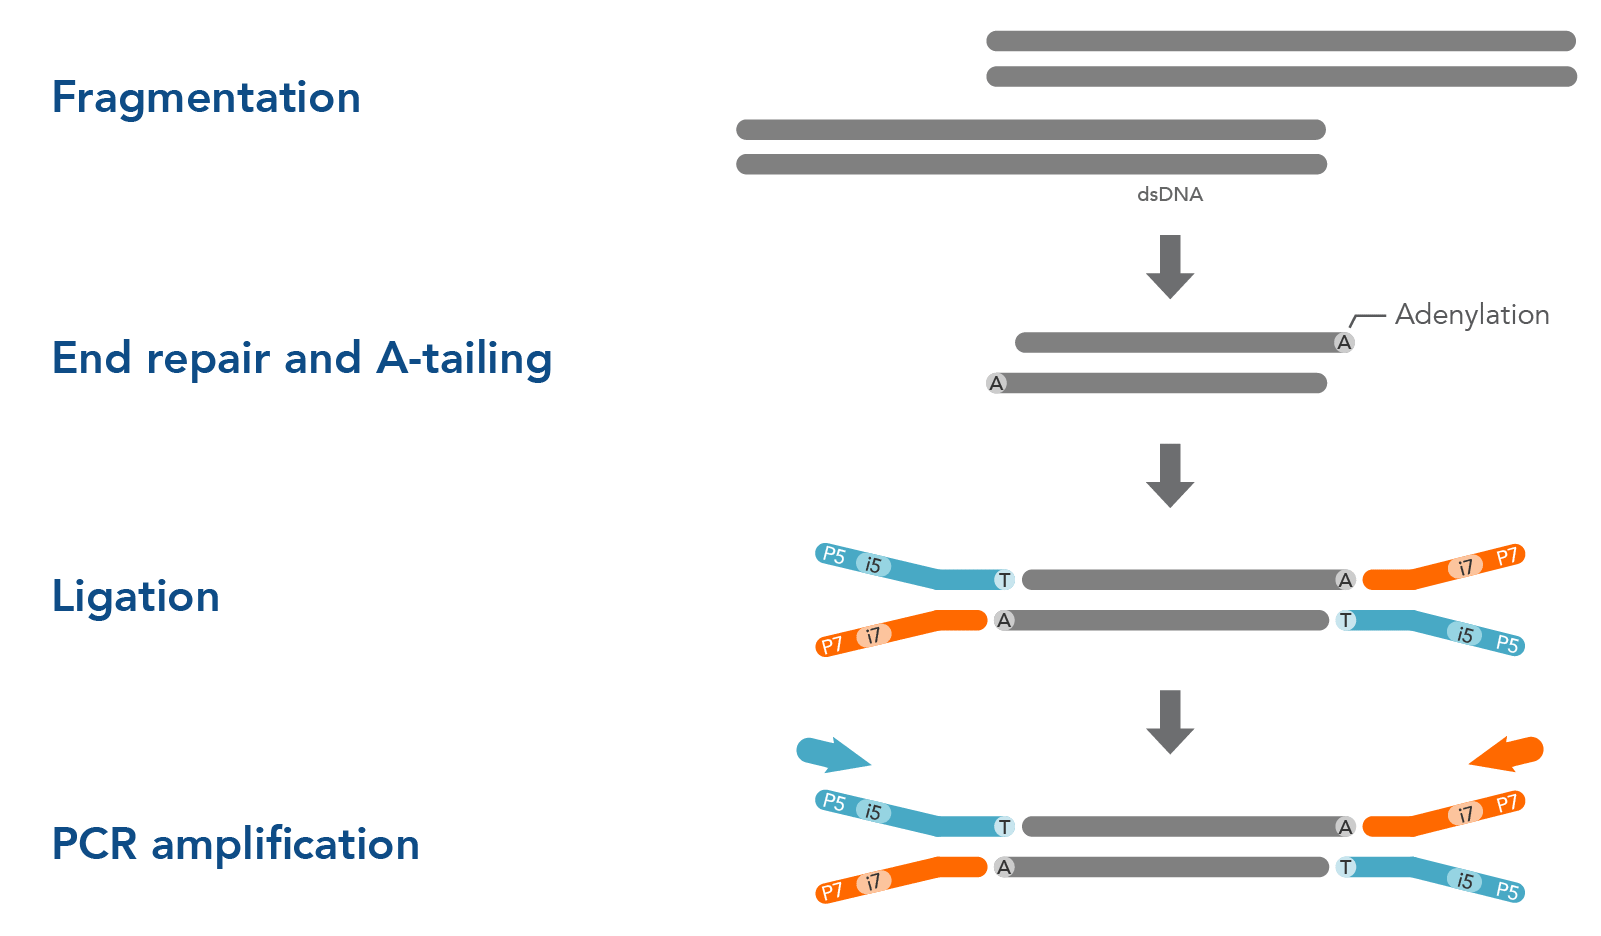
\includegraphics[width = 0.8\textwidth]{figs/19_ng_lib-prep-frag.png}
\caption{Esquema de la preparación de librerías por fragmentación.}
\end{figure}

Las técnicas de fragmentación por ligación incluyen:
\begin{itemize}
\item \textit{Fragmentación física (sonicación)}:
Mediante un sonicador, se aplican ondas sonoras que generan vibración por resonancia, dividiendo el ADN en fragmentos. La frecuencia de las ondas determina el tamaño de los fragmentos obtenidos.
\item \textit{Fragmentación química:}
Se utilizan agentes químicos, como ácidos o bases fuertes, para romper los enlaces fosfodiéster del ADN. Este método es útil en casos donde la epigenética no es relevante, ya que los químicos fuertes pueden modificar las marcas epigenéticas mediante procesos de oxidación o reducción.
\item \textit{Fragmentación enzimática:}
Se emplean endonucleasas, que son enzimas capaces de cortar las cadenas de ADN en puntos específicos, produciendo fragmentos con extremos cohesivos o romos. Este método permite una fragmentación precisa, pero puede introducir sesgos en la representatividad de la librería generada.
\end{itemize}

\begin{figure}[htbp]
\centering
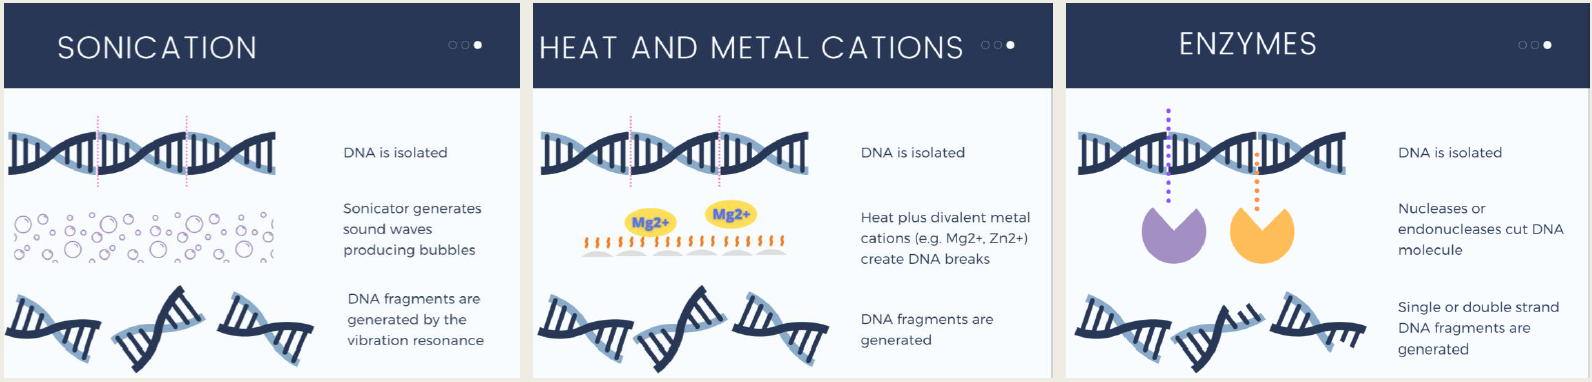
\includegraphics[width = \textwidth]{figs/ligation-methods.png}
\caption{Representación gráfica de los distintos métodos de fragmentación por ligación.}
\end{figure}

\begin{table}[htbp]
\centering
\resizebox{\textwidth}{!}{\begin{tabular}{l | l l l}
& Physical & Chemical & Enzymatic \\ \hline \hline
Pro & Broad range & Well for RNA & Standard lab equipment \\
& Unbiased & & Highly scalable \\
& Less sample variation & Lower input of material \\
& Even sized of fragments & & \\
& No interferences & & \\
& Easy to implement & & \\ \hline
Cons & Expensive equipment & Cations interfere with some seq methods & Fragmentation bias \\
& Loss of material & & Ratio material/enzymes \\
& Modification of bases & & Sample-to-sample variation
\end{tabular}}
\caption{Pros y contras de cada método de fragmentación por ligación}
\end{table}

\item \textbf{Aproximación por tagmentación: }
En este método, se utiliza la enzima tagmentasa, una transposasa que corta la secuencia de ADN e incorpora adaptadores de manera enzimática \footnote{Los transposones son elementos móviles dentro del ADN.}. La tagmentación es rápida y eficiente, pues combina la fragmentación y la adición de adaptadores en un solo paso.

\begin{figure}[htbp]
\centering
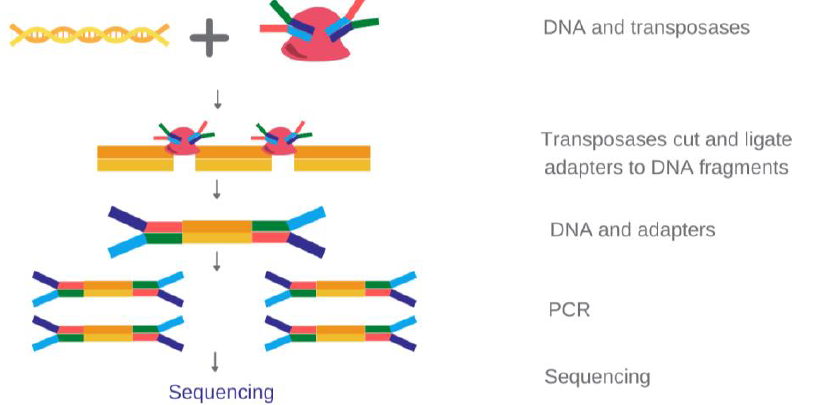
\includegraphics[width = 0.8\textwidth]{figs/tagmentation.png}
\caption{Representación esquemática de la fragmentación por tagmentación.}
\end{figure}
\end{itemize} 

\subsubsection{Reparación de extremos y ligación de adaptadores}
Después de la fragmentación del ADN, es necesario reparar los extremos de los fragmentos. Como la fragmentación no suele producir cortes limpios, los fragmentos generados suelen presentar extremos sobresalientes (overhangs). Para corregir esto, se realiza un tratamiento enzimático con polimerasas, que además añade una adenina (A) en los extremos 3’. Estos extremos, con la adenina añadida, facilitan la ligación de los adaptadores, los cuales suelen tener un overhang de timina (T) para permitir una unión complementaria con los fragmentos de ADN.

\begin{figure}[htbp]
\centering
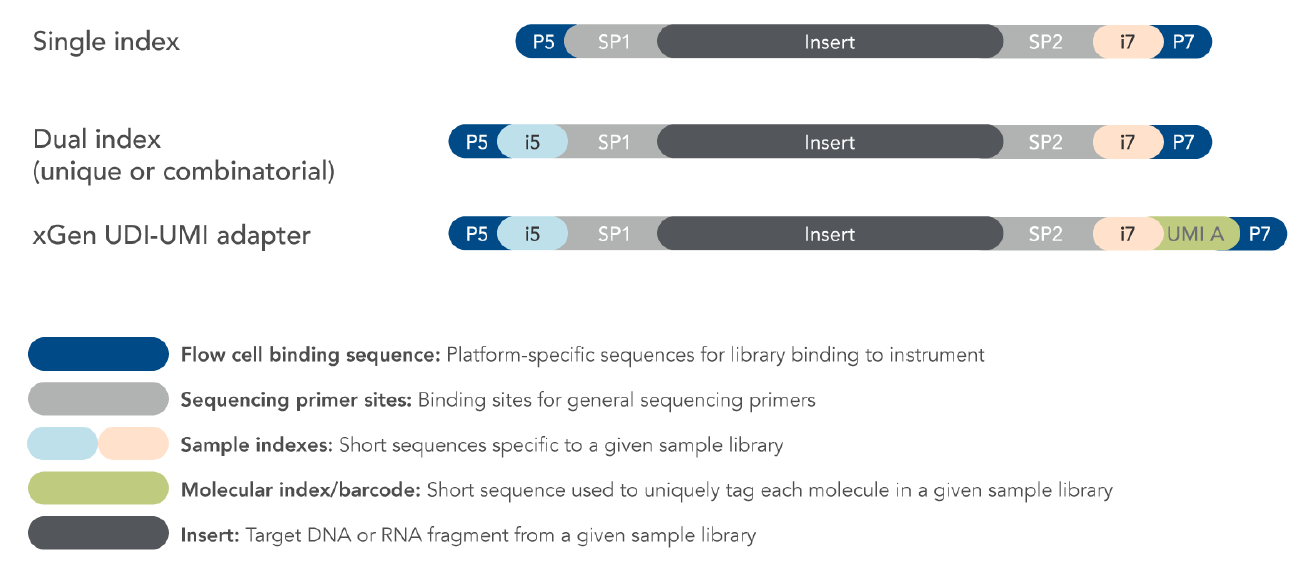
\includegraphics[width = \textwidth]{figs/adaptator.png}
\caption{Representación de los adaptadores en caso de secuenciación simple, dual y UDI-UMI.}
\end{figure}

Los adaptadores empleados en la secuenciación tienen distintas configuraciones. Por lo general, se colocan dos tipos de adaptadores: el adaptador P5 en un extremo y el adaptador P7 en el otro. Esta disposición permite identificar las direcciones de lectura durante el proceso de secuenciación. Además, algunos adaptadores incluyen identificadores moleculares únicos, conocidos como UMIs (Unique Molecular Identifiers), que permiten rastrear de forma única cada molécula de ADN. Durante la amplificación, todas las moléculas con el mismo UMI corresponden a la misma molécula de ADN original. Esto tiene múltiples beneficios:
\begin{itemize}
\item \textbf{Eliminación de duplicados de PCR:} Permite distinguir duplicados generados por PCR de secuencias originales.
\item \textbf{Disminuir el ratio de error:} La lectura de la misma molécula varias veces permite detectar posibles errores generados durante la construcción de la librería o la amplificación. Si diferentes secuencias presentan un UMI idéntico pero difieren en algún nucleótido, se puede deducir que ha habido un error, ya que las secuencias deberían ser idénticas. Esto ayuda a reducir el índice de error y a detectar variantes poco frecuentes.
\end{itemize}

\begin{figure}[htbp]
\centering
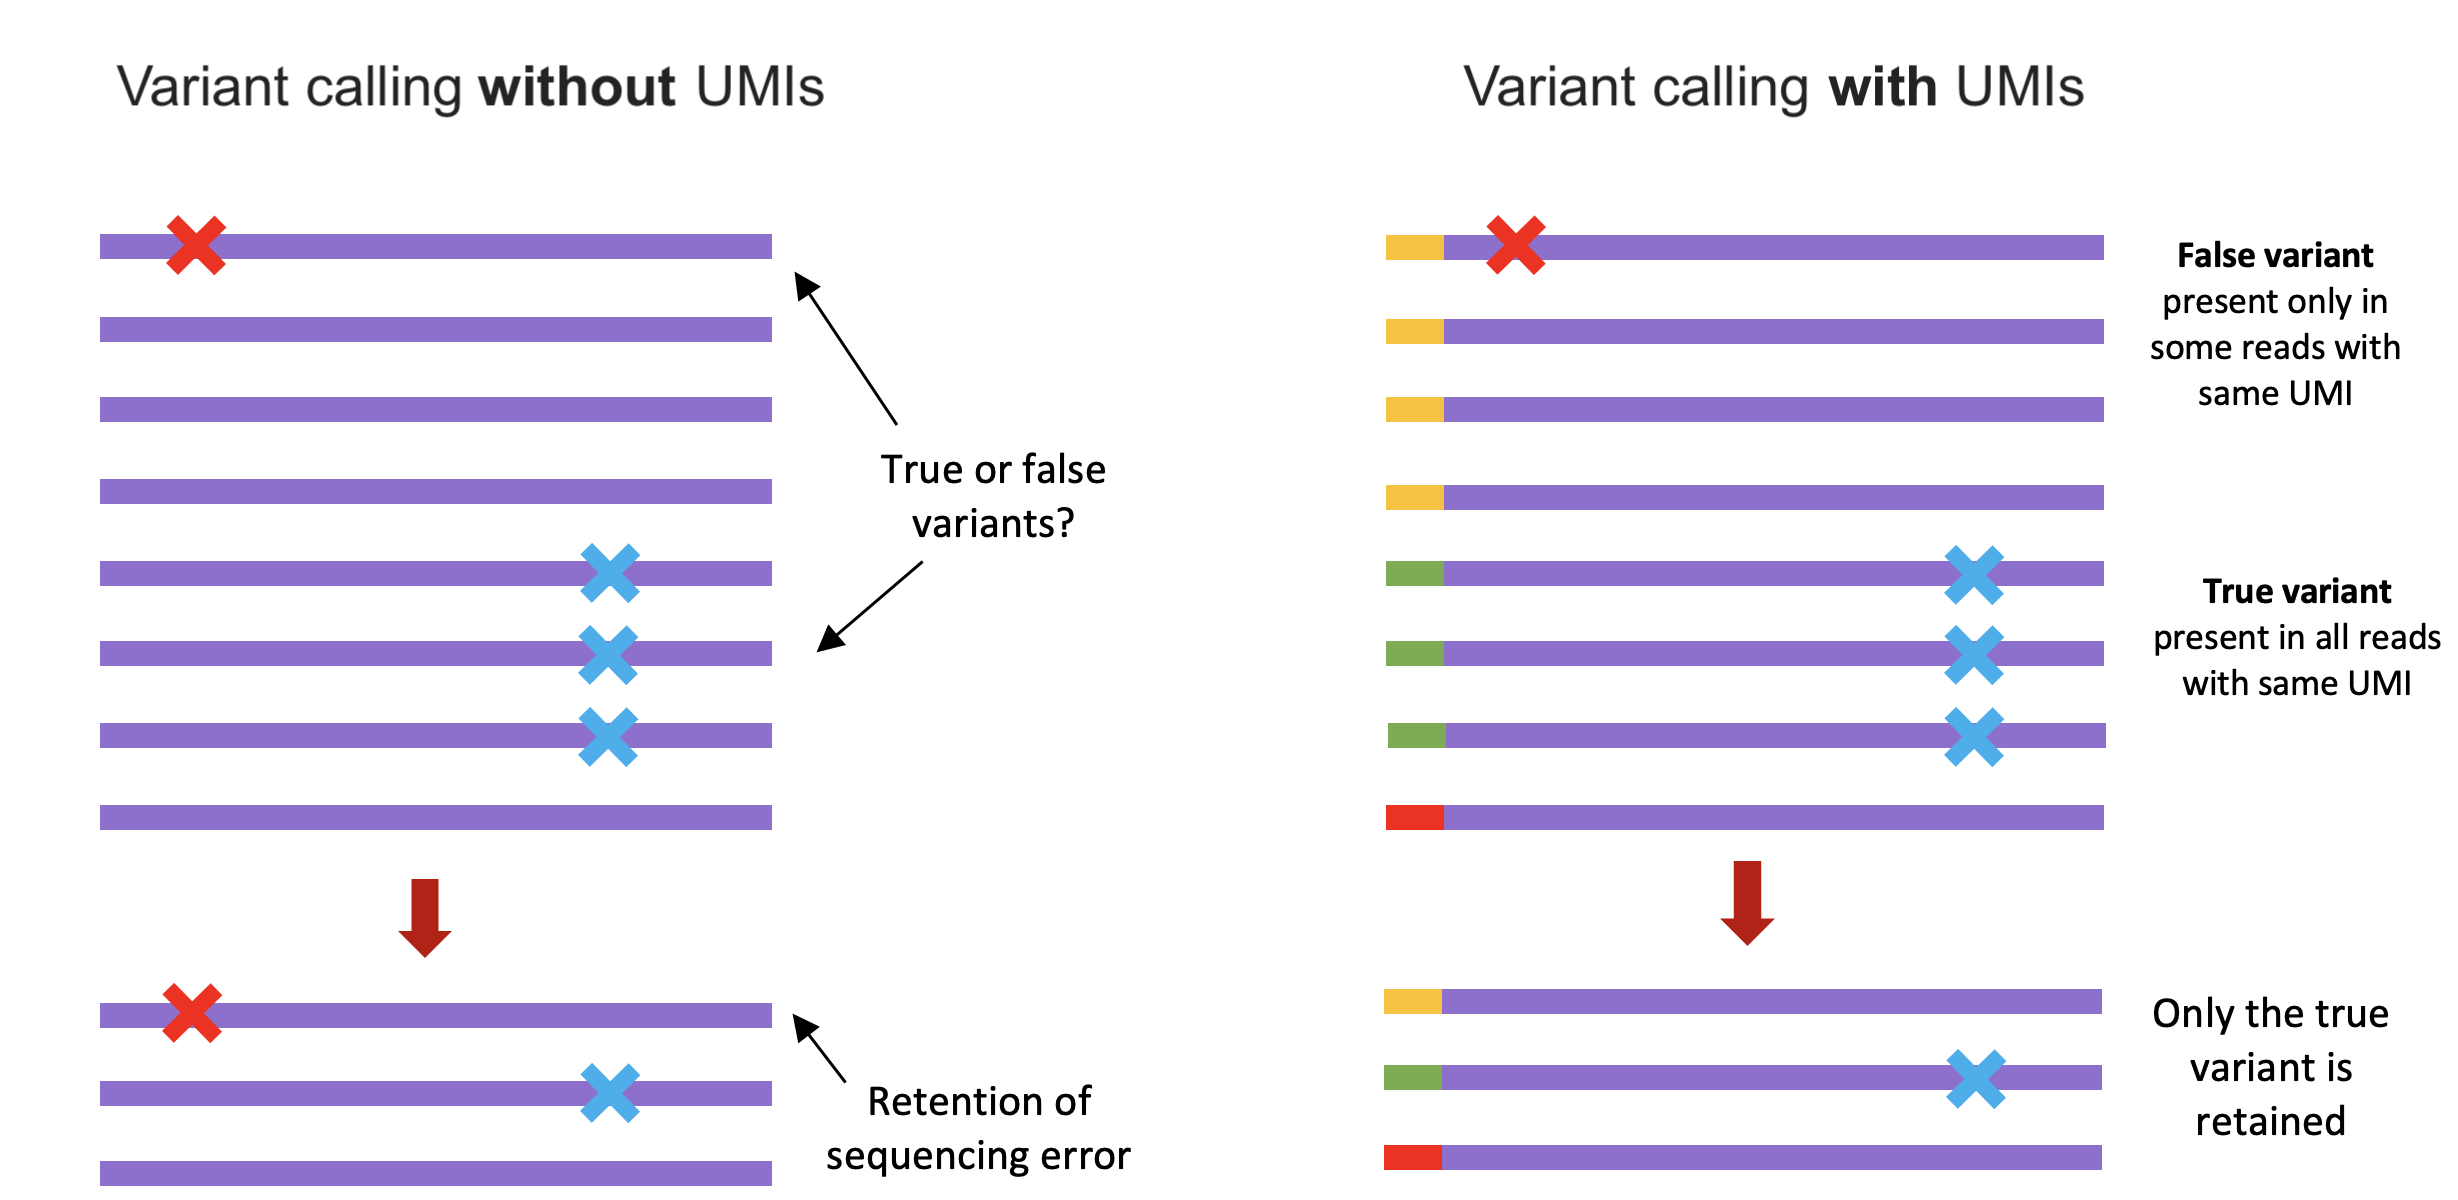
\includegraphics[width = \textwidth]{figs/umi-variants.png}
\caption{Representación de variantes con y sin UMIs.}
\end{figure}

En el método conocido como \textbf{Duplex Sequencing}, se emplean UMIs distintos en ambos extremos del fragmento de ADN. De este modo, durante el análisis de consenso, se pueden identificar las posiciones que muestran concordancia entre ambas hebras y descartar los nucleótidos mutados por error.

\begin{figure}[htbp]
\centering
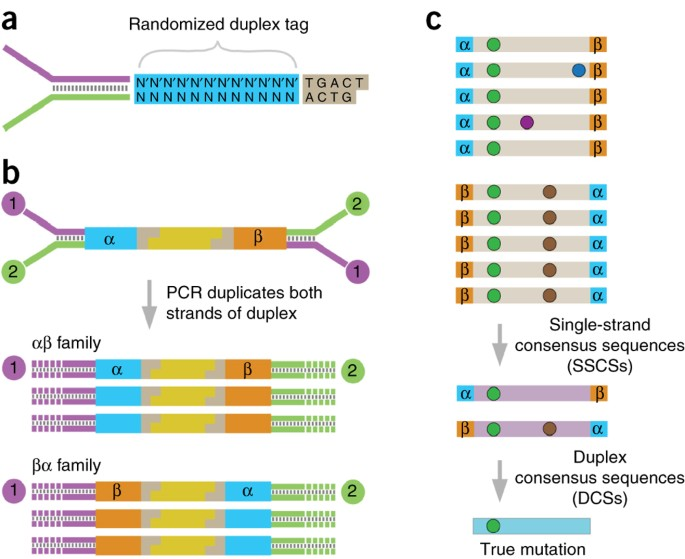
\includegraphics[width = 0.8\textwidth]{figs/duplex-sequencing.jpg}
\caption{Visión general de la secuenciación dúplex. (a) Esquema de un adaptador de secuenciación dúplex, que muestra la etiqueta aleatoria de doble cadena y la secuencia espaciadora invariante. (b) La ligación de los adaptadores con el ADN de la muestra da lugar a una secuencia única de 12 nt en ambos extremos de la molécula. La amplificación por PCR de cada cadena de un dúplex de ADN da lugar a dos productos de PCR distintos pero relacionados. (c) Las lecturas que comparten secuencias únicas de etiquetas $\alpha$ y $\beta$ se agrupan en familias de etiquetas de forma $\alpha \beta$ o $\beta \alpha$, y se crea un SSCS (single-strand consensus sequence) para cada familia de etiquetas. Las mutaciones son de tres tipos diferentes: errores de secuenciación (puntos azules o morados); errores de PCR de primera ronda (puntos marrones); mutaciones verdaderas (puntos verdes). La formación del SSCS elimina el primer tipo de error, pero no los errores de PCR de la primera ronda. La comparación de los SSCS de las familias emparejadas con etiquetas $\alpha \beta$ y $\beta \alpha$, genera un DCS (duplex consensus sequence), que elimina estos errores de PCR de primera ronda. Las mutaciones verdaderas se puntúan si y sólo si están presentes en la misma posición en ambas cadenas del ADN. "Detecting ultralow-frequency mutations by Duplex Sequencing, Nature, 2014"}
\end{figure}

Aunque los métodos basados en UMIs son altamente eficaces para detectar variantes de muy baja frecuencia, su uso es limitado debido a su alto costo, ya que requieren múltiples lecturas de la misma secuencia para asegurar precisión.

\subsubsection{Adaptadores para secuenciación de célula única (single cell)}
En la secuenciación de célula única (Single Cell), se emplean adaptadores y primers que contienen UMIs específicos tanto para cada célula como para cada molécula de ADN. Esto permite diferenciar si las lecturas corresponden a una célula particular y, dentro de esa célula, a una molécula específica. En Single Cell, se utiliza un enfoque de consenso: las lecturas múltiples de la misma molécula permiten generar una secuencia de consenso para mejorar la precisión de los datos.

\begin{figure}[htbp]
\centering
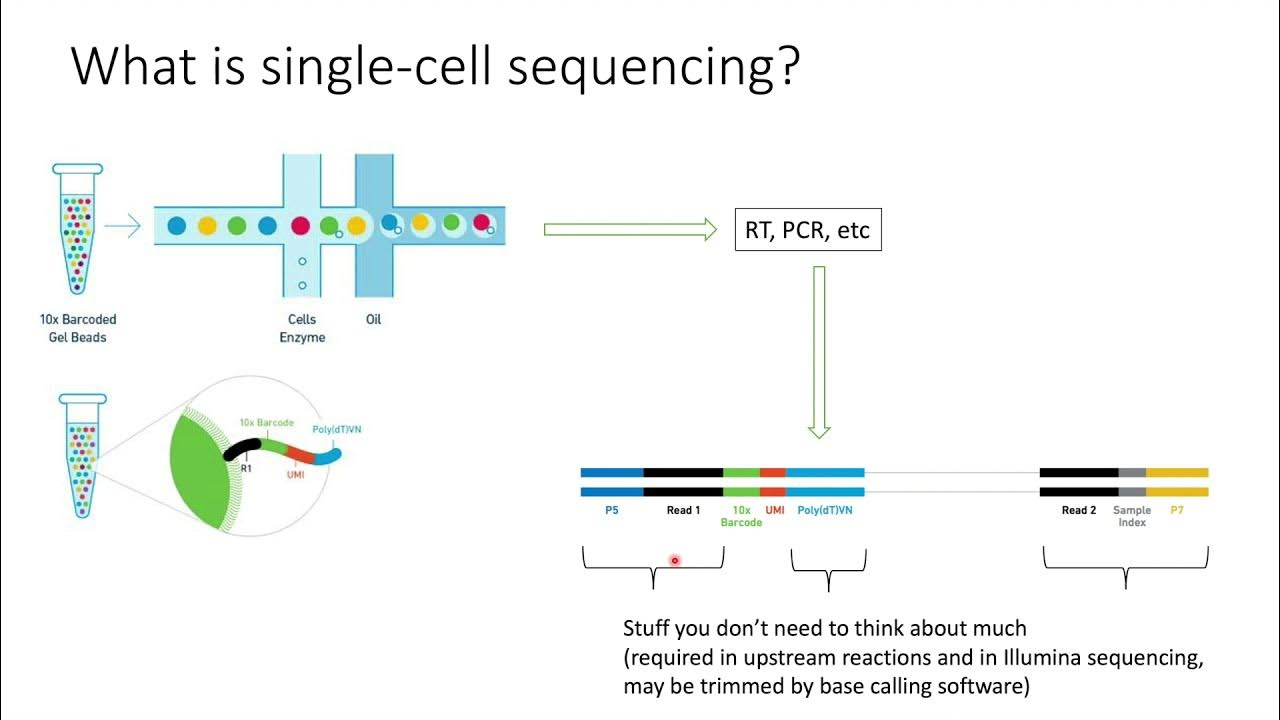
\includegraphics[width = 0.8\textwidth]{figs/single-cell-seq.jpg}
\caption{Descripción esquemática de la generación de GEM (gel beads-in-emulsions) y el código de barras con el flujo de trabajo del chip GEM-X. Los GEM se generan combinando perlas de gel con código de barras, una mezcla maestra que contiene células y aceite de partición en un chip GEM-X 3' o 5'. Para lograr una resolución unicelular, las células se suministran a una dilución límite, de modo que la mayoría ($\approx$90-99\%) de los GEM generados no contienen ninguna célula, mientras que el resto contiene en gran medida una sola célula.}
\end{figure}

La construcción de librerías en Single Cell se realiza mediante chips que permiten el paso de flujo de células individuales junto con liposomas que contienen la mezcla de PCR. Cada mezcla de PCR tiene adaptadores con un barcode específico de célula, pero diferentes barcodes de molécula. Esto permite identificar y diferenciar las células individuales entre sí.

%Glosario
\begin{table}[htbp]
\begin{mdframed}[backgroundcolor=black!10]
    \centering
\textbf{Glosario}
\begin{description}
\item[Adaptadores:] Moléculas cortas de ADN fabricadas artificialmente que se unen a fragmentos de ADN y se utilizan para unirse a la célula de flujo.
\item[Barcoding:] El proceso de identificar muestras de ADN añadiendo índices a los fragmentos de ADN durante la preparación de la librería.
\item[Índice:] Molécula corta de ADN fabricada artificialmente que se utiliza para asignar códigos únicos a las muestras, lo que permite su identificación durante la secuenciación.
\item[Insert:] Fragmento de ADN entre dos adaptadores.
\item[Librería:] Una colección de fragmentos de ADN de tamaño aleatorio procedentes de una muestra determinada para ser secuenciados.
\item[Preparación de librería por ligación:] Método para ligar adaptadores a fragmentos de ADN para ser secuenciados.
\item[Multiplexing:] El proceso de añadir índices a los fragmentos de ADN durante la preparación de la librería.
\item[Oligos:] Moléculas de ADN artificial unidas a la célula de flujo que se unen por complementación a los adaptadores de los fragmentos de ADN.
\item[Lecturas/Reads:] Secuencias de pares de bases obtenidas de fragmentos de ADN.
\item[Preparación de librería por tagmentación:] Método para cortar y ligar adaptadores a fragmentos de ADN utilizando una enzima transposasa.
\item[Transposasa:] Enzima utilizada en la preparación de bibliotecas de marcaje para cortar y ligar adaptadores a fragmentos de ADN.
\end{description}
    \end{mdframed}
\end{table}

\subsection{Formatos de datos}
El formato de archivo usado por los alineadores es generalmente \textbf{FastQ} para las secuencias, aunque \textbf{Fast5} o \textbf{HDF5} también se emplean en algunos casos, especialmente en secuenciación de célula única (single cell), donde se necesita un mayor nivel de detalle en el almacenamiento de datos.

Cuando se trabaja con alineadores, el proceso suele generar un perfil con picos que representan las bases detectadas, a cada uno de los cuales se le asigna un nombre de base. El alineador produce un archivo final que contiene tanto la secuencia de bases asignadas como la calidad de lectura de cada base en un formato codificado llamado \textbf{Phred33}, que usa caracteres ASCII para representar los valores de calidad.

En formatos antiguos, la cabecera de cada secuencia incluía datos detallados, como el nombre del instrumento de secuenciación, el identificador del flowcell, las coordenadas X e Y del clúster, el número de la muestra y el índice del par de lectura. En el formato actual, esta información en la cabecera ha sido simplificada o se presenta de manera distinta.

En cuanto al tipo de secuenciación, se distinguen dos tipos:
\begin{itemize}
\item \textbf{Single-end:} lee la secuencia en una sola dirección.
\item \textbf{Paired-end:} realiza lecturas en ambas direcciones, proporcionando información desde ambos extremos del fragmento de ADN. La secuenciación puede ser solapante (overlapping) para incrementar la evidencia de la secuencia, o no solapante (non-overlapping) cuando se busca mapear estructuras más amplias sin redundancia en los extremos.
\end{itemize}

\begin{figure}[htbp]
\centering
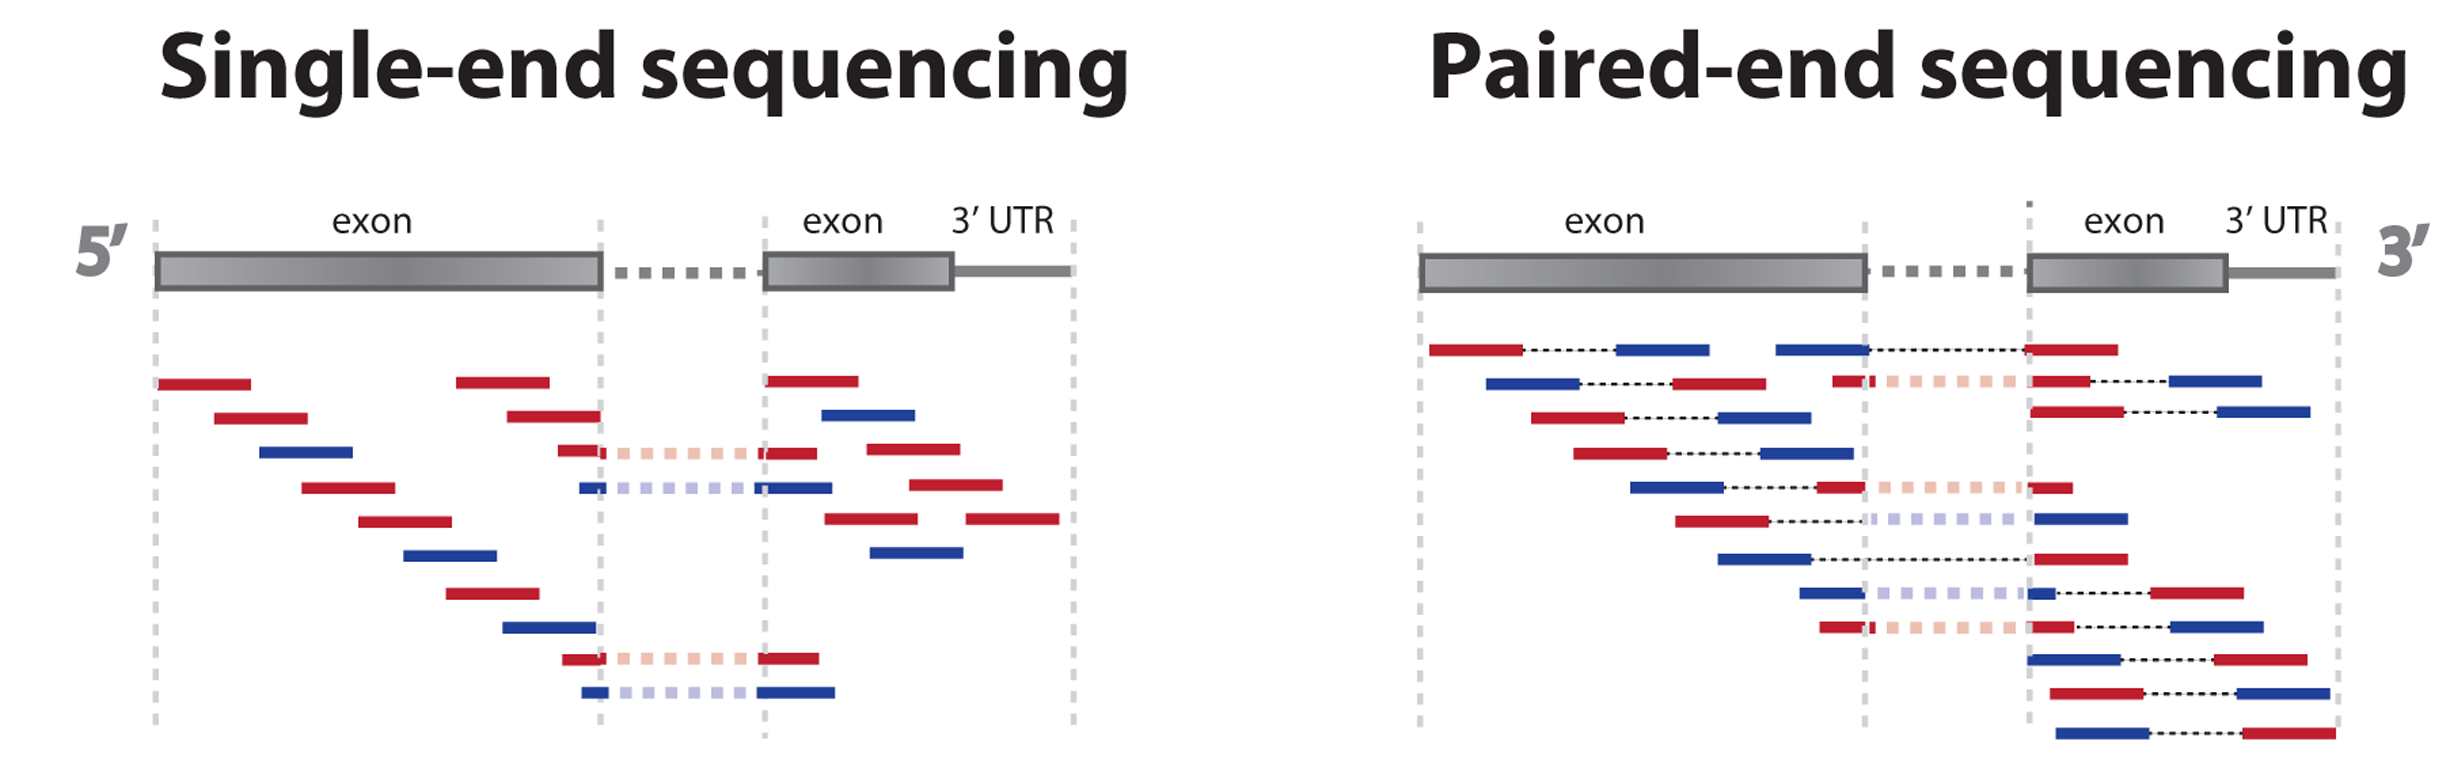
\includegraphics[width = 0.8\textwidth]{figs/singleEndVsPairedEnd.png}
\caption{Representación gráfica de la diferencia entre Single end y Paired end.}
\end{figure}

Durante un experimento de secuenciación, se utiliza un programa llamado \textbf{FastQC} para evaluar la calidad de las bases a lo largo de la lectura mediante una métrica llamada \textbf{Q score}. La visualización de estos resultados suele hacerse a través de diagramas de barras y cajas. Normalmente, la calidad de las bases tiende a disminuir conforme avanzan los ciclos de lectura, pero debe mantenerse dentro de un rango confiable.

\begin{figure}[htbp]
\centering
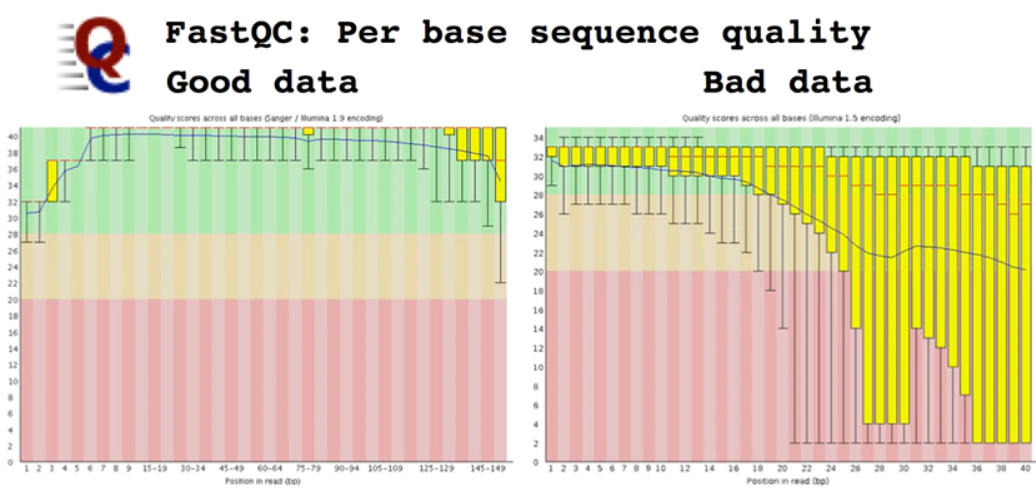
\includegraphics[width = \textwidth]{figs/good-bad-fastq.png}
\caption{La calidad de la secuencia por base, que representa la puntuación Q de la secuencia en crudo, se lee como un gráfico de caja para cada ciclo. Cuanto más alto, mejor, y en la mayoría de los ciclos se observa un descenso característico de la calidad.}
\end{figure}

FastQC proporciona varias métricas clave para evaluar la calidad: 
\begin{itemize} 
\item \textbf{Calidad promedio de la secuencia}: muestra la calidad media de las bases en cada posición. 
\item \textbf{Proporciones de bases por posición}: indica la proporción de bases (A, T, C, G) en cada posición. 
\item \textbf{Contenido de bases por posición}: permite identificar cualquier sesgo en el contenido de bases a lo largo de la secuencia. 
\item \textbf{Contenido GC:} al inicio de la secuenciación, puede haber una variación en el contenido GC debido a la secuencia de los adaptadores, pero si se estabiliza después de las primeras bases, indica una secuenciación correcta y se pueden cortar los primeros nucleótidos. 
\end{itemize}

\subsection{Preprocesamiento y genomas de referencia} 
El preprocesamiento de las lecturas aumenta la calidad de las secuencias, mejora el mapeo, elimina posibles contaminantes y sesgos, y descarta segmentos no informativos.

Las secuencias generadas se comparan con \textbf{genomas de referencia}, que generalmente están en formato \textbf{FASTA}. En estos archivos, los nucleótidos están representados según el código IUPAC para permitir una representación estándar de variaciones. Históricamente, los genomas de referencia se creaban con la información genética de un solo individuo. Sin embargo, hoy en día, se basan en el consenso de los genomas de múltiples individuos, lo que permite identificar variantes y posiciones con alta confianza que difieren entre individuos.

Los genomas de referencia y sus anotaciones se pueden encontrar en sitios como \href{https://hgdownload.soe.ucsc.edu/downloads.html}{UCSC Genome Browser}. Es importante tener en cuenta las diferencias en las anotaciones genómicas entre repositorios europeos y americanos, ya que pueden variar en la numeración y anotación de los cromosomas.

\subsection{Alineamientos y mapeo}
El alineamiento es el proceso de comparar secuencias de ADN, ARN o proteínas para identificar regiones de similitud, lo cual puede revelar relaciones funcionales, estructurales o evolutivas entre especies. Los objetivos principales del alineamiento son:
\begin{itemize}
\item Determinar el grado de homología para inferir relaciones filogenéticas
\item Identificar dominios funcionales
\item Comparar el gen con sus productos asociados
\item Encontrar posiciones homólogas entre secuencias
\item Identificar diferencias entre secuencias similares
\end{itemize}

\subsubsection{Alineamiento vs Mapeo}
Aunque a menudo se usan indistintamente, el alineamiento y el mapeo tienen diferencias importantes:
\begin{itemize}
\item \textbf{Alineamiento:} Cada posición de la secuencia de consulta se compara exhaustivamente con una secuencia de referencia para evaluar su precisión en cada sitio.
\item \textbf{Mapeo:} El objetivo es encontrar los loci más probables en la referencia donde una secuencia podría alinearse, priorizando eficiencia en velocidad y memoria.
\end{itemize}

Existen programas diseñados específicamente para el mapeo, llamados alineadores de corta lectura, que permiten configuraciones de mapeo como mapeo único, mapeo múltiple o mapeo con calidades parciales. Dependiendo del tipo de secuenciación, se emplean diferentes alineadores:
\begin{itemize}
\item \textbf{Para ADN:} Novoalign, Bowtie2, BWA
\item \textbf{Para ARN:} RSEM, Salmon, Sleuth
\end{itemize}

\subsubsection{Algoritmos de mapeo por hashing}
El mapeo inicia con una etapa de \textbf{indexación del genoma}, un proceso intensivo en tiempo y memoria que se realiza solo una vez por genoma de referencia y por programa. En esta fase, los algoritmos de alineamiento utilizan técnicas como \textbf{hashing} o \textbf{índices} basados en \textbf{k-mers} (subsecuencias de longitud fija). Con una ventana móvil, se anotan las posiciones de cada k-mer en la secuencia de referencia.

Posteriormente, las lecturas se comparan con el diccionario de k-mers para localizar sus posiciones sin usar una ventana móvil adicional. A continuación, se construye un "árbol de posibilidades" que evalúa la compatibilidad de cada lectura con la referencia. Si una mutación en la lectura no coincide con la referencia, el k-mer no estará en el índice, y se buscarán los k-mers más cercanos, evaluando el mapping quality según el número de errores (mismatches) y la distancia de edición. El objetivo es minimizar los gaps (espacios sin coincidencias) para mejorar la precisión del alineamiento.

\begin{figure}[htbp]
\centering
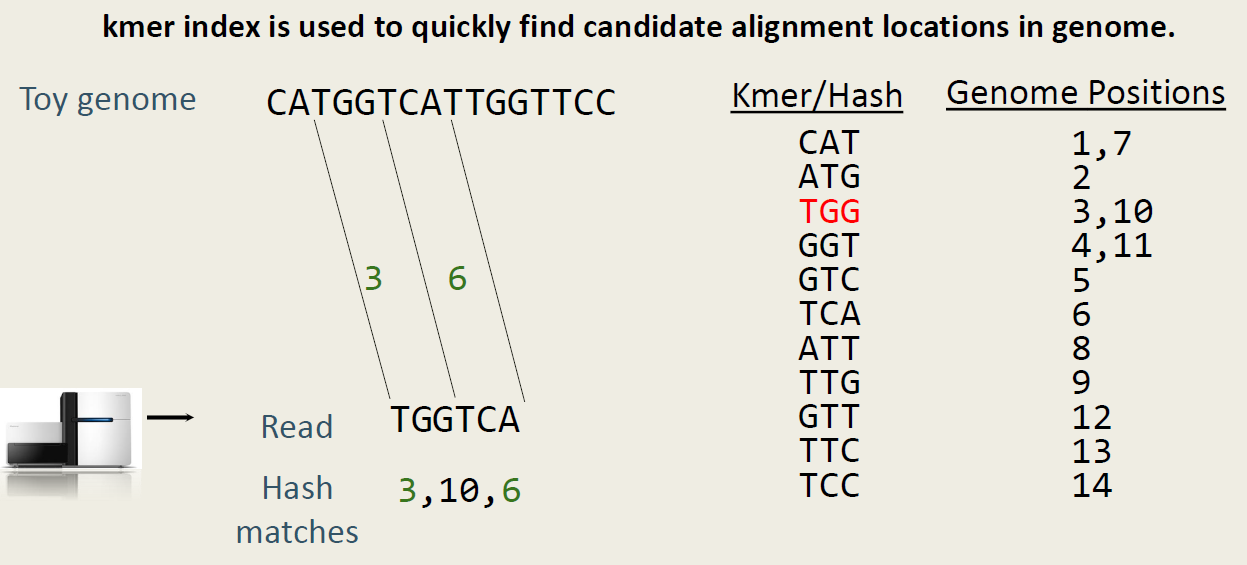
\includegraphics[width = \textwidth]{figs/hash-mapping.png}
\caption{Mapeado basados en hash o índices. El primer paso es obtener el hash o índice del genoma de referencia completo. A continuación, se utilizan esos índices para mapear (es decir, encontrar sitios de alineamiento) las lecturas.}
\end{figure}

\subsubsection{Transformación de Burrows-Wheeler (BWT)}
La \textbf{transformación de Burrows-Wheeler} es un método de compresión que permite realizar búsquedas rápidas de alineamiento en el genoma de referencia, optimizando el rendimiento de los alineadores.

\subsubsection{Estados de lecturas post-mapeo y mapping quality}
Una vez mapeadas las lecturas al genoma de referencia, estas pueden clasificarse en distintos estados:
\begin{itemize}
\item \textbf{Lecturas no mapeadas:} No encuentran ninguna coincidencia en la referencia.
\item \textbf{Lecturas con mapeo único:} Mapean en una sola posición. Normalmente se trabaja con estas lecturas.
\item \textbf{Lecturas con mapeo múltiple (multimappers):} Mapean en varias posiciones. Se distinguen primarios y secundarios en función de la puntuación de mapeo.
\end{itemize}

Existen opciones para reportar todos los alineamientos, solo los mejores, o aquellos que superan un umbral de calidad específico.

La calidad de mapeo usa la misma escala Phred33 que las calidades de lectura, y los resultados de alineación se almacenan en formatos SAM, BAM o CRAM:
\begin{itemize}
\item \textbf{SAM:} Formato de texto plano.
\item \textbf{BAM:} Versión binaria de SAM.
\item \textbf{CRAM:} Similar a BAM, pero usado principalmente por el EBI, optimizado para almacenar datos de forma compacta.
\end{itemize}

Los formatos SAM y BAM se pueden convertir entre sí mediante la herramienta \textbf{samtools}, que permite especificar el nivel de compresión.

La cabecera del archivo BAM comienza con \@ y almacena metadatos como la versión de SAM, la ordenación, los contigs y la información general del mapeo. Los datos de alineación incluyen: 
\begin{itemize} 
\item Nombre de la lectura 
\item Flag: Indica si la lectura está mapeada o no, entre otras propiedades. 
\item Cromosoma: Donde se ha mapeado la lectura. 
\item Posición inicial en el cromosoma 
\item Calidad de mapeo 
\item CIGAR string: Codificación de los eventos de alineamiento (match, mismatch, inserciones, deleciones). Por ejemplo, un CIGAR de 3M1D2M1I1M indica que hay 3 match, 1 deleción, 2 match, 1 inserción y 1 match.
\item Información sobre el mapeo del par: En caso de secuenciación paired-end, se incluye la ubicación de la pareja de la lectura. 
\end{itemize}

